%\documentclass[wcp,gray]{jmlr} % test grayscale version
 %\documentclass[wcp]{jmlr}% former name JMLR W\&CP
\documentclass[pmlr]{jmlr}% new name PMLR (Proceedings of Machine Learning)

 % The following packages will be automatically loaded:
 % amsmath, amssymb, natbib, graphicx, url, algorithm2e

 %\usepackage{rotating}% for sideways figures and tables
\usepackage{longtable}% for long tables

 % The booktabs package is used by this sample document
 % (it provides \toprule, \midrule and \bottomrule).
 % Remove the next line if you don't require it.
\usepackage{booktabs}
 % The siunitx package is used by this sample document
 % to align numbers in a column by their decimal point.
 % Remove the next line if you don't require it.
\usepackage[load-configurations=version-1]{siunitx} % newer version
 %\usepackage{siunitx}

\makeatletter
\def\set@curr@file#1{\def\@curr@file{#1}} %temp workaround for 2019 latex release
\makeatother

 % The following command is just for this sample document:
\newcommand{\cs}[1]{\texttt{\char`\\#1}}

 % Define an unnumbered theorem just for this sample document:
\theorembodyfont{\upshape}
\theoremheaderfont{\scshape}
\theorempostheader{:}
\theoremsep{\newline}
\newtheorem*{note}{Note}

 % change the arguments, as appropriate, in the following:
\jmlrvolume{}
\jmlryear{2020}
\jmlrworkshop{Machine Learning for Healthcare}

% Short headings should be running head and authors last names
% \ShortHeadings{A Really Awesome MLHC Article}{Lastname, PhD and Lastname, MD}
% \firstpageno{1}

\title[Comparisons Between HMC and MAP For Precision Medicine]{Comparisons Between Hamiltonian Monte Carlo and Maximum A Posteriori For A Bayesian Model For Apixaban Induction Dose \& Dose Personalization}

%\author{\Name{A. Demetri Pananos}
%       \Email{apananos@uwo.ca}\\ 
%       \addr Department of Epidemiology and Biostatistics\\
%       Western University\\
%		London, Ontario, Canada
%       \AND
%       \Name{Daniel J. Lizotte}
%       \Email{dlizotte@uwo.ca}\\ 
%       \addr Department of Epidemiology and Biostatistics\\
%       Department of Computer Science\\
%       Western University\\
%       London, Ontario, Canada} 
%
%\editor{Editor's name}

%My imports
\usepackage[noabbrev]{cleveref}
\usepackage{tikz}
\usetikzlibrary{bayesnet}
\usepackage{rotating}
\begin{document}

\maketitle

\begin{abstract}
Precision medicine’s slogan is “right drug -- right patient -- right time.” Implicit in the slogan is ``right dose''; however, determining the right dose for any one patient can be challenging when dose-response data are limited. Bayesian methods, with their ability to explicitly incorporate prior information to supplement limited data, have been proposed as a solution to this problem. Although Hamiltonian Monte Carlo (HMC) is a leading methodology for inference in Bayesian models because of its ability to capture posterior distributions with high fidelity, dose personalization studies commonly use simpler Maximum A Posteriori (MAP) inference methods. The impact of the choice of inference engine on dose decision-making has not been explored.   To better understand this issue, we perform a simulation study characterizing the differences between inferences made via MAP and HMC for personalized dosing strategies. The simulation study uses a new Bayesian pharmacokinetic model for apixaban pharmacokinetics written in an open source Bayesian language; the model code and posterior summaries of all parameters will be publicly available. We demonstrate that the differences between HMC and MAP are non-trivial and can greatly affect the choices surrounding dose selection for personalized medicine.

\end{abstract}

%I like to break apart the sections in this way so that editing and debugging is not
% a complete cluster fuck as it usually is in LaTeX
\section{Introduction}

Precision medicine’s slogan is ``right drug -- right patient -- right time''.  Implicit in the slogan is ``right dose''; however, determining the right dose for any one patient can be challenging. The anticoagulant Warfarin offers a good example of these challenges; physicians choose an initial dose based on guidelines and their own experience. They then closely monitor the patient’s International Normalised Ratio (INR), which measures how long it takes blood to clot, and in response they adjust the dose over time.

Pharmacokinetic and statistical models of how drugs behave within an individual can alleviate some of these challenges by predicting the effects of different doses based on patient covariates. In some studies \citep{schwarz2008genetic,Sohrabi2017-zv, Caldwell2007-mi}  a cohort of patients will have an appropriate maintenance doses determined empirically and these are then regressed onto patient covariates.  In others \citep{ohara2019differences,Zhu2017-rk, Xue2017-mp}  patient pharmacokinetics are directly modeled and can be simulated under different dosing regimens to find an appropriate dose.  In both cases, uncertainty in the models can be assessed and can help guide clinical decisions as to what dose is best or what dose to try next.

Both types of  models can provide guidance for individual patients, but only when there is enough data so that the models are accurate and reliable. For personalized pharmacokinetics-based dosing, this amount of data is rarely available in practice.  Obtaining sufficient data to learn a patient’s pharmacokinetic parameters requires a lengthy observation period which few patients are willing or capable of committing to. Population pharmacokinetic models could be used in place of a patient’s pharmacokinetics, but treating the patient as “average” is precisely what precision medicine seeks to improve upon.

In many contexts where limited data area available, Bayesian methods with informative priors have been proposed.  Model priors allow analysts to specify their beliefs about model parameters prior to seeing a new patient's data, and to combine those beliefs with new observations to form personalized predictive models.  This allows models to ``hit the ground running'' so to speak, and makes use of all available data to support decision-making.  To use all but the simplest of Bayesian models for decision-making requires computational approximation techniques to obtain model estimates and predictions. Several approaches exist for generating approximate samples from the posterior distribution, with Hamiltonian Monte Carlo (HMC) being considered the gold standard \citep{Neal1996-vn, Matthew_D_Hoffman2014-in, Carpenter2017-qf, Tripuraneni2017-oh}. Despite HMC being the preferred method by theorists and applied Bayesians alike, methods like Maximum A Posteriori (MAP), in which the posterior mode is computed via optimization and then a Laplace approximation is performed, continue to be used in population Bayesian pharmacokinetic studies as late as 2020 \citep{Brooks2016-li, Nguyen2016-pg,  Preijers2019-kc,Stifft2020-uq}. HMC and MAP are two different approaches with different strengths and different theoretical motivations. Naturally, this raises questions regarding how decisions in personalized medicine may be affected by the use of different methods for performing inference, even using the same model and data. We seek to answer these questions by developing a new, high-fidelity Bayesian pharmacokinetic model and then investigating the impact of the choice of inference method on precision medicine decisions. 

\subsection*{Generalizable Insights about Machine Learning in the Context of Healthcare}

The main methodological insight we gained was that \textit{although predictions made by HMC and MAP may appear to be very similar according to common error metrics, they can lead to very different personalized dosing decisions.} The main contributions of this paper are as follows: 

\begin{enumerate}
\item A new Bayesian model for apixaban pharmacokinetics written in an open source Bayesian language.  We make the model code and posterior summaries of all parameters publicly available at \href{https://github.com/Dpananos/PKBayes}{https://github.com/Dpananos/PKBayes}.

\item A simulation study demonstrating that inferences made via MAP and HMC lead to very different dosing strategies.

\item An induction dosing model for apixaban based on desired trough concentration level after a first dose.
\end{enumerate}





\section{Background}
\subsection*{Pharmacokinetic Modelling}

Broadly, pharmacokinetics is the study of the dynamics of a mass of drug in the body and is concerned with the absorption, distribution, metabolism, and excretion of that drug.  Differential equations (equations which relate the derivative of an unknown function to itself) are often used to describe how these dynamics evolve over time. The differential equation models in pharmacokinetics are called “compartmental models” as they idealize different parts of the body as compartments from which drug can flow in and out at rates proportional to how much drug is presently in that compartment. If the differential equation is not too complex, the solution can be written in terms of analytic functions.  In the case where the differential equation can not be solved in terms of analytic functions, a rich literature of numerical techniques exist to approximate the solution to within quantifiable precision. In either case, estimation of model parameters is of  interest as they represent pharmacokinetic measures, such as the volume of distribution or rate constants for which the drug is absorbed into/excreted out of a compartment. If the parameters for such a model are known, we can use the models to make predictions about drug concentration as a function of time and dose. This in turn can be used to select a dose that meets given criteria about what the concentration function should look like.

Parameter estimation for these models can be done in both frequentist and Bayesian frameworks.  In a Bayesian framework, parameter estimation begins by specifying a prior distribution which reflects the knowledge of parameters before seeing data. Once data are observed, Bayes’ rule can be used to get the posterior distribution.  This distribution provides information about what parameter values have most plausibly generated the observed data.  By virtue of being a probability distribution, the posterior can be summarized by expectations to get point estimates of model parameters. Shown in \cref{fig:fig1} is a visual summary of how Bayes’ rule and Bayesian modelling of pharmacokinetics works using pseudodata. The leftmost panel is our prior distribution.  Each concentration curve results from specific combinations of parameters for the model which are believed to be plausible before seeing data.  Once data are observed (the middle panel), application of Bayes’ rule yields the rightmost panel.  Concentration curves in this panel correspond to combinations of parameters which have most plausibly generated the data, resulting in concentration curves which have most plausibly generated the data. Note that in this setting, because we have many measurements, the pharmacokinetic model is well-determined and the posterior uncertainty is small. Except in very simple cases, the integrals required to evaluate the posterior quickly become intractable, thus computational approximations are required to fit Bayesian models.
%
\begin{figure} [h!]
	\centering
	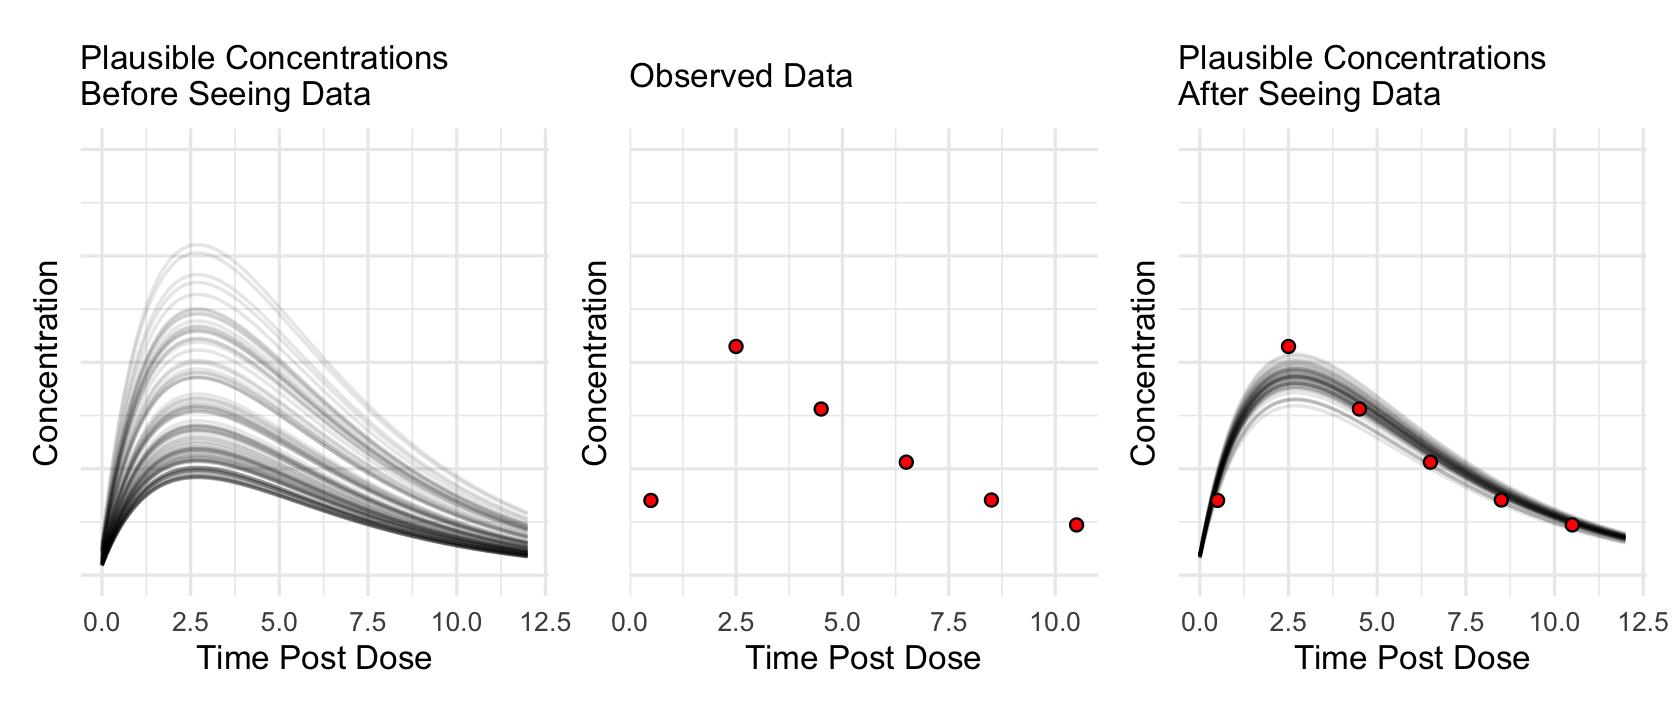
\includegraphics[width=\linewidth]{figs/fig_1}
	\caption{A demonstration of a Bayesian workflow for pharmacokientic models.  The leftmost panel represents the prior.  Each curve corresponds to a unique set of model parameters which induce each concentration function.  In the center panel is the data observed from a single patient.  Conditioning on this data yields the rightmost panel.  Each curve corresponds to a unique set of model parameters drawn from the posterior distribution.} 
	\label{fig:fig1}
\end{figure}
%
\subsection*{Dosing Decisions}

Vitamin K antagonists, such as the popular oral anticoagulant Warfarin, are known to have narrow therapeutic windows as well as drug and food interaction. Determination of a maintenance dose is consequently a procedure with frequent monitoring and followup, with some sources recommending monitoring daily or every other day until the INR stabilizes for two days.  The narrow therapeutic window forces investigators to also consider the pharmacodynamics (the study of the onset, intensity, and duration of the drug response and how these are related to the concentration of the drug at its site of action) of Warfarin in addition with the pharmacokinetics when determining dose size as concentration of the drug alone is not sufficient to infer the antithrombotic effect in patients. The introduction of factor Xa inhibitors like apixaban has alleviated some of the difficulties in prescribing anticoagulants.  Factor Xa inhibitors have been shown to have lower risk for bleeding than Warfarin in patients with atrial fibrillation \cite{vinogradova2018risks} and also allow for fixed dosing without frequent monitoring INR. Furthermore, unlike Warfarin, the pharmacodynamic effect of apixaban on clotting is closely correlated with the concentration in the plasma \cite{Byon2019-gf}, making pharmacokinetic modelling more informative on antithrombotic effect as compared to Warfarin.  However, as of writing this paper there is little information on the therapeutic window, making selecting dose sizes large enough to avoid thromboembolism difficult. Furthermore, studies have demonstrated that inter-patient variability of apixaban plasma concentrations is much higher than was initially believed {\bf CITE MARKUS}. In this work, we develop personalized dosing whose goal is to find the minimum dose that avoids plasma concentrations that are too low. 


\section{Methods}

\subsection*{Bayesian Model}

To achieve our three objectives of 1) developing a new Bayesian pharmacokinetic model for apixaban, 2) investigating the impact of MAP versus HMC inference on dosing decisions and 3) developing an induction dosing model for apixaban, we fit a hierarchical mixed effects model of apixaban pharmacokinetics using data from \cite{Beaton2018-el}.  Thirty-six participants were given 5 mg of apixaban and 100 ml of water in a fasted state. Blood plasma concentrations of apixaban were recorded over the course of 12 hours.



\begin{table}[htb]
	\centering
	\caption{Summary of data from  \cite{Beaton2018-el}. } 
	\label{tab:my table} 
	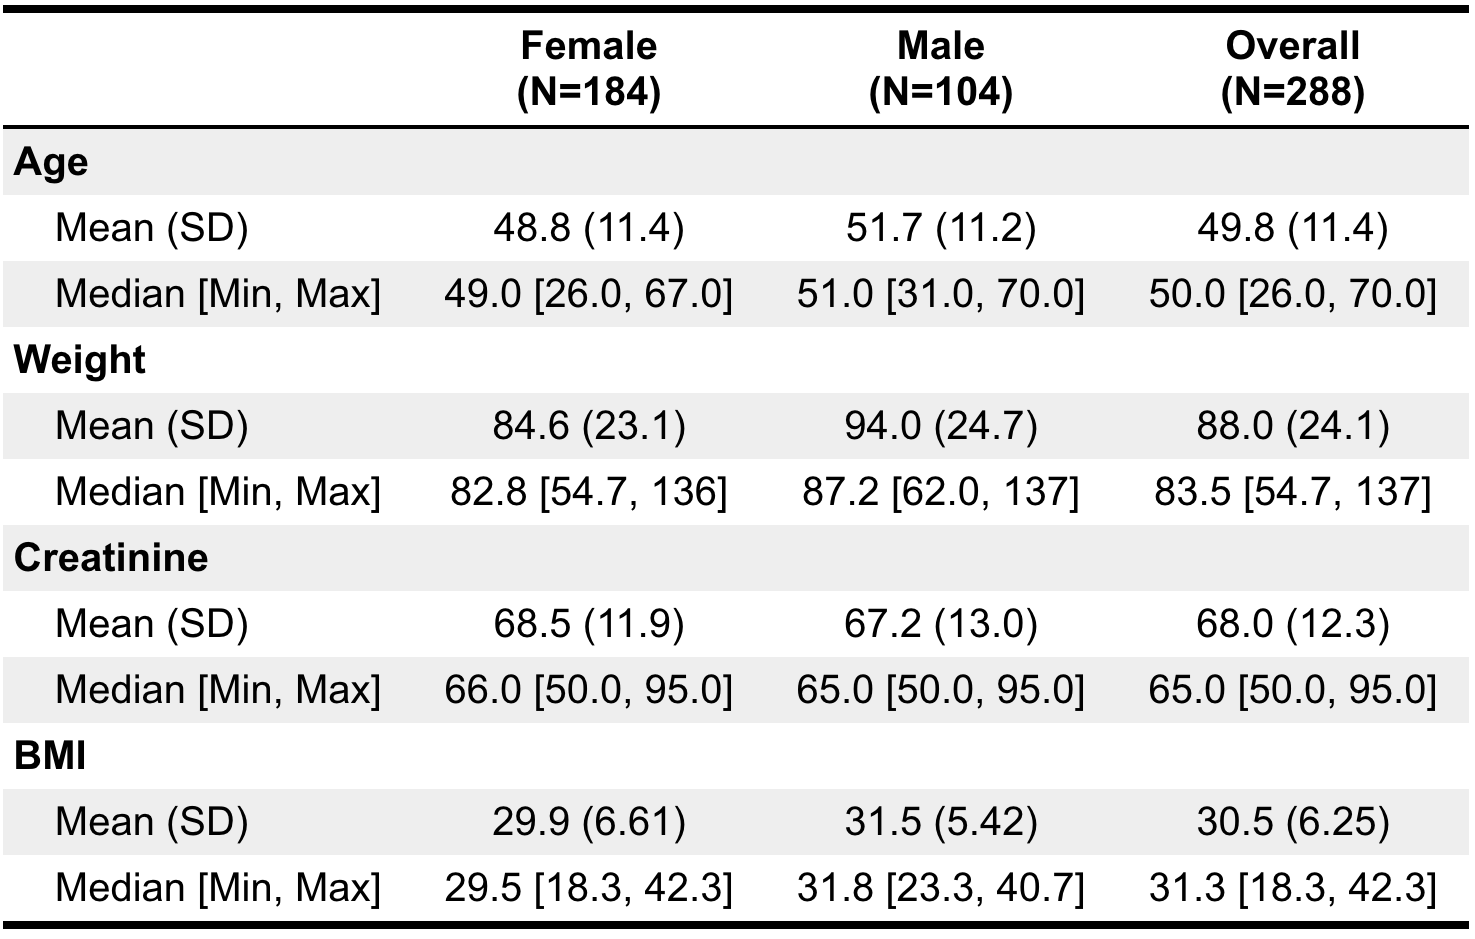
\includegraphics[width=0.7\linewidth]{figs/table1}
\end{table}


\noindent Since participants were given a single dose of apixaban in a fasted state, we use a single-compartment pharmacokinetic model with first order absorption and elimination.  The solution to the differential equation describing mass transit, and consequently the concentration function, is then


\begin{equation} \label{eq:eq_1}
y(t) =  \begin{cases}  \dfrac{F \cdot D}{\mathit{Cl}} \dfrac{k_e \cdot k_a}{k_e - k_a}\Bigg( e^{-k_a (t-\delta)} - e^{-k_e(t-\delta)} \Bigg)  & \delta \leq t\\\\ 0 & \mbox{else} \end{cases}
\end{equation}

\noindent Here, $D$ is the size of the dose in mg, $F$ is the bioavailability (fixed to 0.5 for apixaban \cite{Byon2019-gf}), $\mathit{Cl}$ is the clearance rate in units litres per hour, $k_a$ is the rate constant of absorption into the volume of distribution in units 1/hours, and $k_e$ is the elimination rate constant in units 1/hours. We include a time delay, $\delta$, to relax the assumption that absorption begins immediately after ingestion.  Parameters are considered as random effects, with some population mean and variance (which is estimated from the data). 

Priors for $k_e$ and $k_a$ are not defined explicitly.  Rather, our model puts priors on the time to max concentration, which can be expressed as a function of the parameters in \cref{eq:eq_1}

\begin{equation}\label{eq:eq_2}
 t_{\mathit{max}} = \dfrac{\ln(k_a) - \ln(k_e)}{k_a - k_e}
\end{equation}

\noindent and on the ratio between $k_e$ and $k_a$, which we call $\alpha$

\begin{equation}\label{eq:eq_3}
\alpha  = \dfrac{k_e}{k_a} \>.
\end{equation}

\noindent We choose to place a prior on the quantity $\alpha$ because it arises when non-dimensionalizing \citep{Lin1988-pr} the differential equation governing mass transit of the drug in and out of the volume of distribution.  The plasma concentration function is a version of the “flip-flop” model \citep{Wakefield1996-yy, Salway2008-gi}, since different parameterizations of this model can yield the same curve, leading to model un-identifiability. To ensure the model is identifiable, we require $k_e<k_a$ as has been done in previous Bayesian analyses of this model \citep{Wakefield1996-yy, Salway2008-gi}. This requirement bounds $\alpha$ to the unit interval.  In principle, information on the elimination rate constant could be obtained by performing a linear regression on the log concentration values in the latter half of the concentration profiles where the drug is being eliminated from the body. To preserve as much data as possible for model fitting, we forgo this approach.  These two sets of equations are used to parameterize the absorption and elimination rate constants as follows
\begin{align}
	k_a &= \dfrac{1}{t_{\mathit{max}}} \dfrac{\ln(\alpha)}{\alpha-1} \label{eq:eq_4} \\
	k_e &= k_a \alpha \label{eq:eq_5}
\end{align}

Time to max concentration values for patient $j$ are drawn from a log normal distribution

\begin{equation}\label{eq:eq_6}
t_{\mathit{max}, j} \vert \mu_t, \sigma_t \sim \operatorname{LogNormal}(\mu_t, \sigma_t)
\end{equation}

\noindent and $\alpha$ is drawn from a weakly informative beta prior to prevent degenerate cases when $\alpha$  is 0 or 1

\begin{equation}\label{eq:eq_7}
\alpha_j \sim \operatorname{Beta}(2,2)  \>.
\end{equation}

\noindent The rate constants for patient $j$,  $k_{e,j}$ and $k_{a,j}$, are determined from \cref{eq:eq_4,eq:eq_5}. The clearance rate is modelled hierarchically

\begin{equation}\label{eq:eq_8}
\mathit{Cl}_j \vert \mu_{\mathit{Cl}}, \sigma_{\mathit{Cl}}  \sim \operatorname{LogNormal}(\mu_{\mathit{Cl}}, \sigma_{\mathit{Cl}}) \>.
\end{equation}

\noindent Each patient is observed to have a non-zero concentration at time 0.5, so the time delay for each patient is no larger than 0.5 hours.  We place a beta prior on the delay

\begin{equation}\label{eq:eq_9}
\delta_j \vert \phi, \kappa \sim \operatorname{Beta}(\phi / \kappa, (1-\phi) / \kappa)
\end{equation}

\noindent and multiply delta by 0.5 in our model to ensure the maximum delay is 0.5 hours.  Here, $\phi$ is the mean of this beta distribution and $\kappa$ determines the precision of the distribution. Shown in \cref{net} is a Bayes net to exposit model structure at a high level.

\begin{figure}[h!]
	\centering
	\begin{tikzpicture}
	
	\node[latent](phi){$\phi$};
	\node[latent, right=of phi](kappa){$\kappa$};
	\node[latent, right = of kappa](s_t){$\sigma_t$};
	\node[latent, right = of s_t](m_t){$\mu_t$};
	\node[latent, right = of m_t](s_cl){$\sigma_{\mathit{Cl}}$};
	\node[latent, right = of s_cl](m_cl){$\mu_{\mathit{Cl}}$};
	
	\node[latent, below = of kappa](delta){$\delta$};
	\node[latent, right = of delta](alpha){$\alpha$};
	\node[latent, below = of m_t](tmax){$t_{\mathit{max}}$};
	\node[latent, below = of s_cl](cl){$\mathit{Cl}$};
	
	\node[obs, below = of alpha](t){$t$};
	\node[obs, right = of t](y){$y$};
	\node[latent, right = of t, xshift = 3.25cm](sig){$\sigma_y$};
	
	\edge{phi}{delta};
	\edge{kappa}{delta};
	
	\edge{s_t}{tmax};
	\edge{m_t}{tmax};
	\edge{s_cl}{cl};
	\edge{m_cl}{cl};
	
	\edge{delta}{y};
	\edge{alpha}{y};
	\edge{tmax}{y};
	\edge{cl}{y};
	\edge{t}{y};
	\edge{sig}{y};
	
	\plate{t_y_pairs}{(t)(y)}{$i=1\dots 8$};
	\plate{patient_level}{(t_y_pairs)(delta)(alpha)(tmax)(cl)}{$j = 1 \dots 36$};
	\end{tikzpicture}
	
	
	\caption{Graphical description of the data generating process for our model.  The data consist of 36 patients, indexed by $j$.  Each of the $j$ patients are observed a total of 8 times, with each observation index by $i$.  The data are generated by drawing random variables from their appropriate distribution at the top level and then drawing child random variables directly there after.  As an example, $\phi$ and $\kappa$ are drawn, which are then used to draw the $\delta_j$, which are then used to draw each of the 8 concentration values, $y_i$ for each of the $j$ patients.}
	\label{net}
\end{figure}

\subsection*{Priors for Model Hyperparameters}

Estimates of the time to max concentration for apixaban place the population median $t_{\mathit{max}}$ near 3.3 hours post dose  \citep{Byon2019-gf}. Assuming the median and the mean are similar, this provides information for $\mu_t$ and so we use specify 

\begin{equation}\label{eq:eq_10}
 p(\mu_t) = \operatorname{Normal}(\log(3.3), 0.25)
\end{equation}

\noindent The standard deviation of the prior for $\mu_t$ was selected via prior predictive checks in which profiles are drawn and priors are assessed as realistic or not.  We choose to err on the side of caution and inflate the uncertainty in this estimate to account for population differences between the measured patients in the data and the patients used in studies to determine the estimates of $t_{\mathit{max}}$. The population variability of $t_{\mathit{max}}$ was modeled as

\begin{equation}\label{eq:eq_11}
p(\sigma_t) = \operatorname{Gamma}(10,100)
\end{equation}

\noindent Using these priors, we recover similar median, min, and max $t_{\mathit{max}}$ values as reported by \cite{Byon2019-gf}. Similarly, we model the population mean and variability for the clearance rate as

\begin{align}
	p(\mu_{\mathit{Cl}}) &= \operatorname{Normal}(\log(3.3), 0.15) \label{eq:eq_12} \\
	p(\sigma_{\mathit{Cl}}) &= \operatorname{Gamma}(15, 100) \label{eq:eq_13}
\end{align}

\noindent so that population estimates of the mean clearance rate are near 3.3 litres per hour with inflated uncertainty to account for possible population differences. We use weakly informative priors for $\phi$ and $\kappa$ which induces an approximately uniform prior on $\delta$.

\begin{align}
	 p(\phi) &= \operatorname{Beta}(20,20) \label{eq:eq_14}\\
	 p(\kappa) &= \operatorname{Beta}(20,20)  \label{eq:eq_15}
\end{align}

The tools used to measure the concentration of apixaban are believed to be within 10\% of the real concentration.  This implies that the observational model is heteroskedastic. We use a log-normal likelihood so that positivity of observed concentrations and heteroskedasticity are respected. We place a lognormal prior on the likelihood’s variability with

\begin{align}
	p(\sigma_y)  &= \operatorname{LogNormal}(\ln(0.1), 0.2) \label{eq:eq_16}\\
	C_{j}(t) \vert \mathit{Cl}_{j}, k_{a,j}, k_{a,j}, \delta_j &\sim \operatorname{LogNormal}(\ln(y(t)), \sigma_y)  \label{eq:eq_17}
\end{align}


\subsection*{Model Fitting and Diagnostics}

For HMC, prior/posterior predictive checks and model fitting was performed using Stan \citep{Carpenter2017-qf} to draw from the prior/posterior.  Twelve chains were initialized and run for 4000 iterations each (1000 for warmup allowing the Markov chain the opportunity to find the correct target distribution and 3000 to use as samples from the posterior). Stan monitors several diagnostics none of which detected problematic HMC behavior\footnote{0 divergences, all Gelman-Rubin diagnostics $<1.01$, smallest effective sample size ratio 16\%.}.

We use Stan’s optimization capabilities to compute the MAP estimates.  The L-BFGS optimizer was used to find the posterior mode.  The optimizer terminated when either 10,000 iterations had been performed or when the value of the objective function stopped changing within a tolerance of 1e-10. Once the mode was located, 10,000 samples from the Laplace approximation to the posterior were obtained. Constrained parameters were transformed to the appropriate space before sampling.

\subsection*{Posterior Summarization and Generating New Data}

Once our model was fit on the pharmacokinetic data, the marginal posteriors were summarized to create priors for the new model.  Parameters for these priors were determined by using maximum likelihood on the posterior samples.  The priors for the new model are as follows:

\begin{align}
	\mu_{\mathit{Cl}} &\sim \operatorname{Normal}(1.64, 0.09)  \label{eq:eq_18} \\
	\sigma_{\mathit{Cl}} &\sim \operatorname{LogNormal}(-0.94, 0.11)  \label{eq:eq_19} \\
	\mu_{t} &\sim \operatorname{Normal}(0.97, 0.05)   \label{eq:eq_20} \\
	\sigma_{t} &\sim \operatorname{LogNormal}(-1.40, 0.12)  \label{eq:eq_21} \\
	\alpha_j &\sim \operatorname{Beta}(2,2)  \label{eq:eq_22} \\
	\sigma_y &\sim \operatorname{LogNormal}(-1.76, 0.12)  \label{eq:eq_23}
\end{align}

\noindent Lognormal distributions were used to respect positivity of some parameters.  The posterior predictive distribution of the model fit to the data from \cite{Byon2019-gf} was then used to simulate 100  pseudopatients.  The time delay, $\delta$ was not used to generate these data as $\delta$ does not affect the overall shape of the concentration function, it merely shifts if right.  The model with the priors defined by \crefrange{eq:eq_18}{eq:eq_23} was then refit on the 100  pseudopatients in order to examine differences between HMC and MAP in a “best case” scenario. The pseudopatients were sampled between 0.5 and 12.0 hours after ingestion in increments of 0.5. Draws from the posterior were used to predict latent concentration for each patient at times 0.75 to 11.75 in increments of 0.5.

\subsection*{Determination of a Personalized Dose}

The results from both  HMC and MAP yield samples from the approximate posterior of $\mathit{Cl}_{j}$, $k_{e,j}$, $k_{a,j}$, and $\delta_j$ for each of the $j$ patients.  For any given posterior sample, these parameters can be combined to compute a predicted concentration for patient $j$ at time $t$ by using \cref{eq:eq_1}.   We determine a personalized dose size by evaluating the pseudopatients’ concentration function under different dose sizes $D$ and then computing posterior probabilities of failing to surpass concentration thresholds.  When we have posterior samples, \cref{eq:eq_1} turns into a function of the dose size and time conditioned on patient. 


We perform two experiments to compare HMC and MAP.  In our first experiment, we determine the posterior probability of failing to exceed a concentration of 20 ng/ml 12 hours post dose for each pseudopatient across a variety of dose sizes. We choose 20 ng/ml as our threshold for this experiment because the median concentration at 12 hours post dose  in the data from \cite{Beaton2018-el} is approximately 20 ng/ml. In our second experiment, we determine the posterior probability that the max concentration fails to exceed 80 ng/ml.  We choose 80 ng/ml as our threshold for this experiment because the median max concentration in the data is 79 ng/ml (though it is important to note that it is unlikely that these patients were observed exactly at the time which the peak concentration was achieved).  These quantities represent two different ways of assessing a patient's risk of being below a given threshold.  The chosen threshold is arbitrary, but our method generalizes to any threshold.  For each experiment, the risks are computed across a grid of dose sizes of 0 mg to 60 mg, yielding risk as a function of dose size.  For each pseudopatient, we interpolate these estimates using a monotone Hermite spline and then invert the risk curve; the inverted risk curve maps risk to dose. This allows us to determine a dose size which produces a specified risk level.



\section{Results}
\subsection*{Bayesian Model}

Diagnostic plots for Bayesian model fit to the real apixaban data is shown in \cref{fig:fig3}.  Posterior population prediction intervals (that is, the result of integrating out the random effect of each patient) of the observed concentration are realistic and to the eye appear similar to the observed data (top left of \cref{fig:fig3}).  Residual plots (observed minus posterior mean) indicate homogeneity of variance on the log scale, which is consistent both with expert knowledge on the measurement process and the likelihood we choose (bottom left of \cref{fig:fig3}). Predicted concentrations tend to agree with observed concentrations (top right of \cref{fig:fig3}), and posterior predictive draws have similar empirical cumulative distribution functions as the observed data (bottom right of \cref{fig:fig3} ). In \cref{fig:fig4}, we show concentration functions obtained from draws from our prior distribution as well as two patients with best and worst fit as measured by mean absolute percentage error (best: 3.29\%, worst: 26.4\%). Because our HMC diagnostics do not indicate problematic behaviour in the Markov chains, and because the model diagnostics indicate adequate fit, we believe the obtained model’s posterior predictive distribution is adequate for simulation of pseudopatients.


\begin{figure}
	\centering
	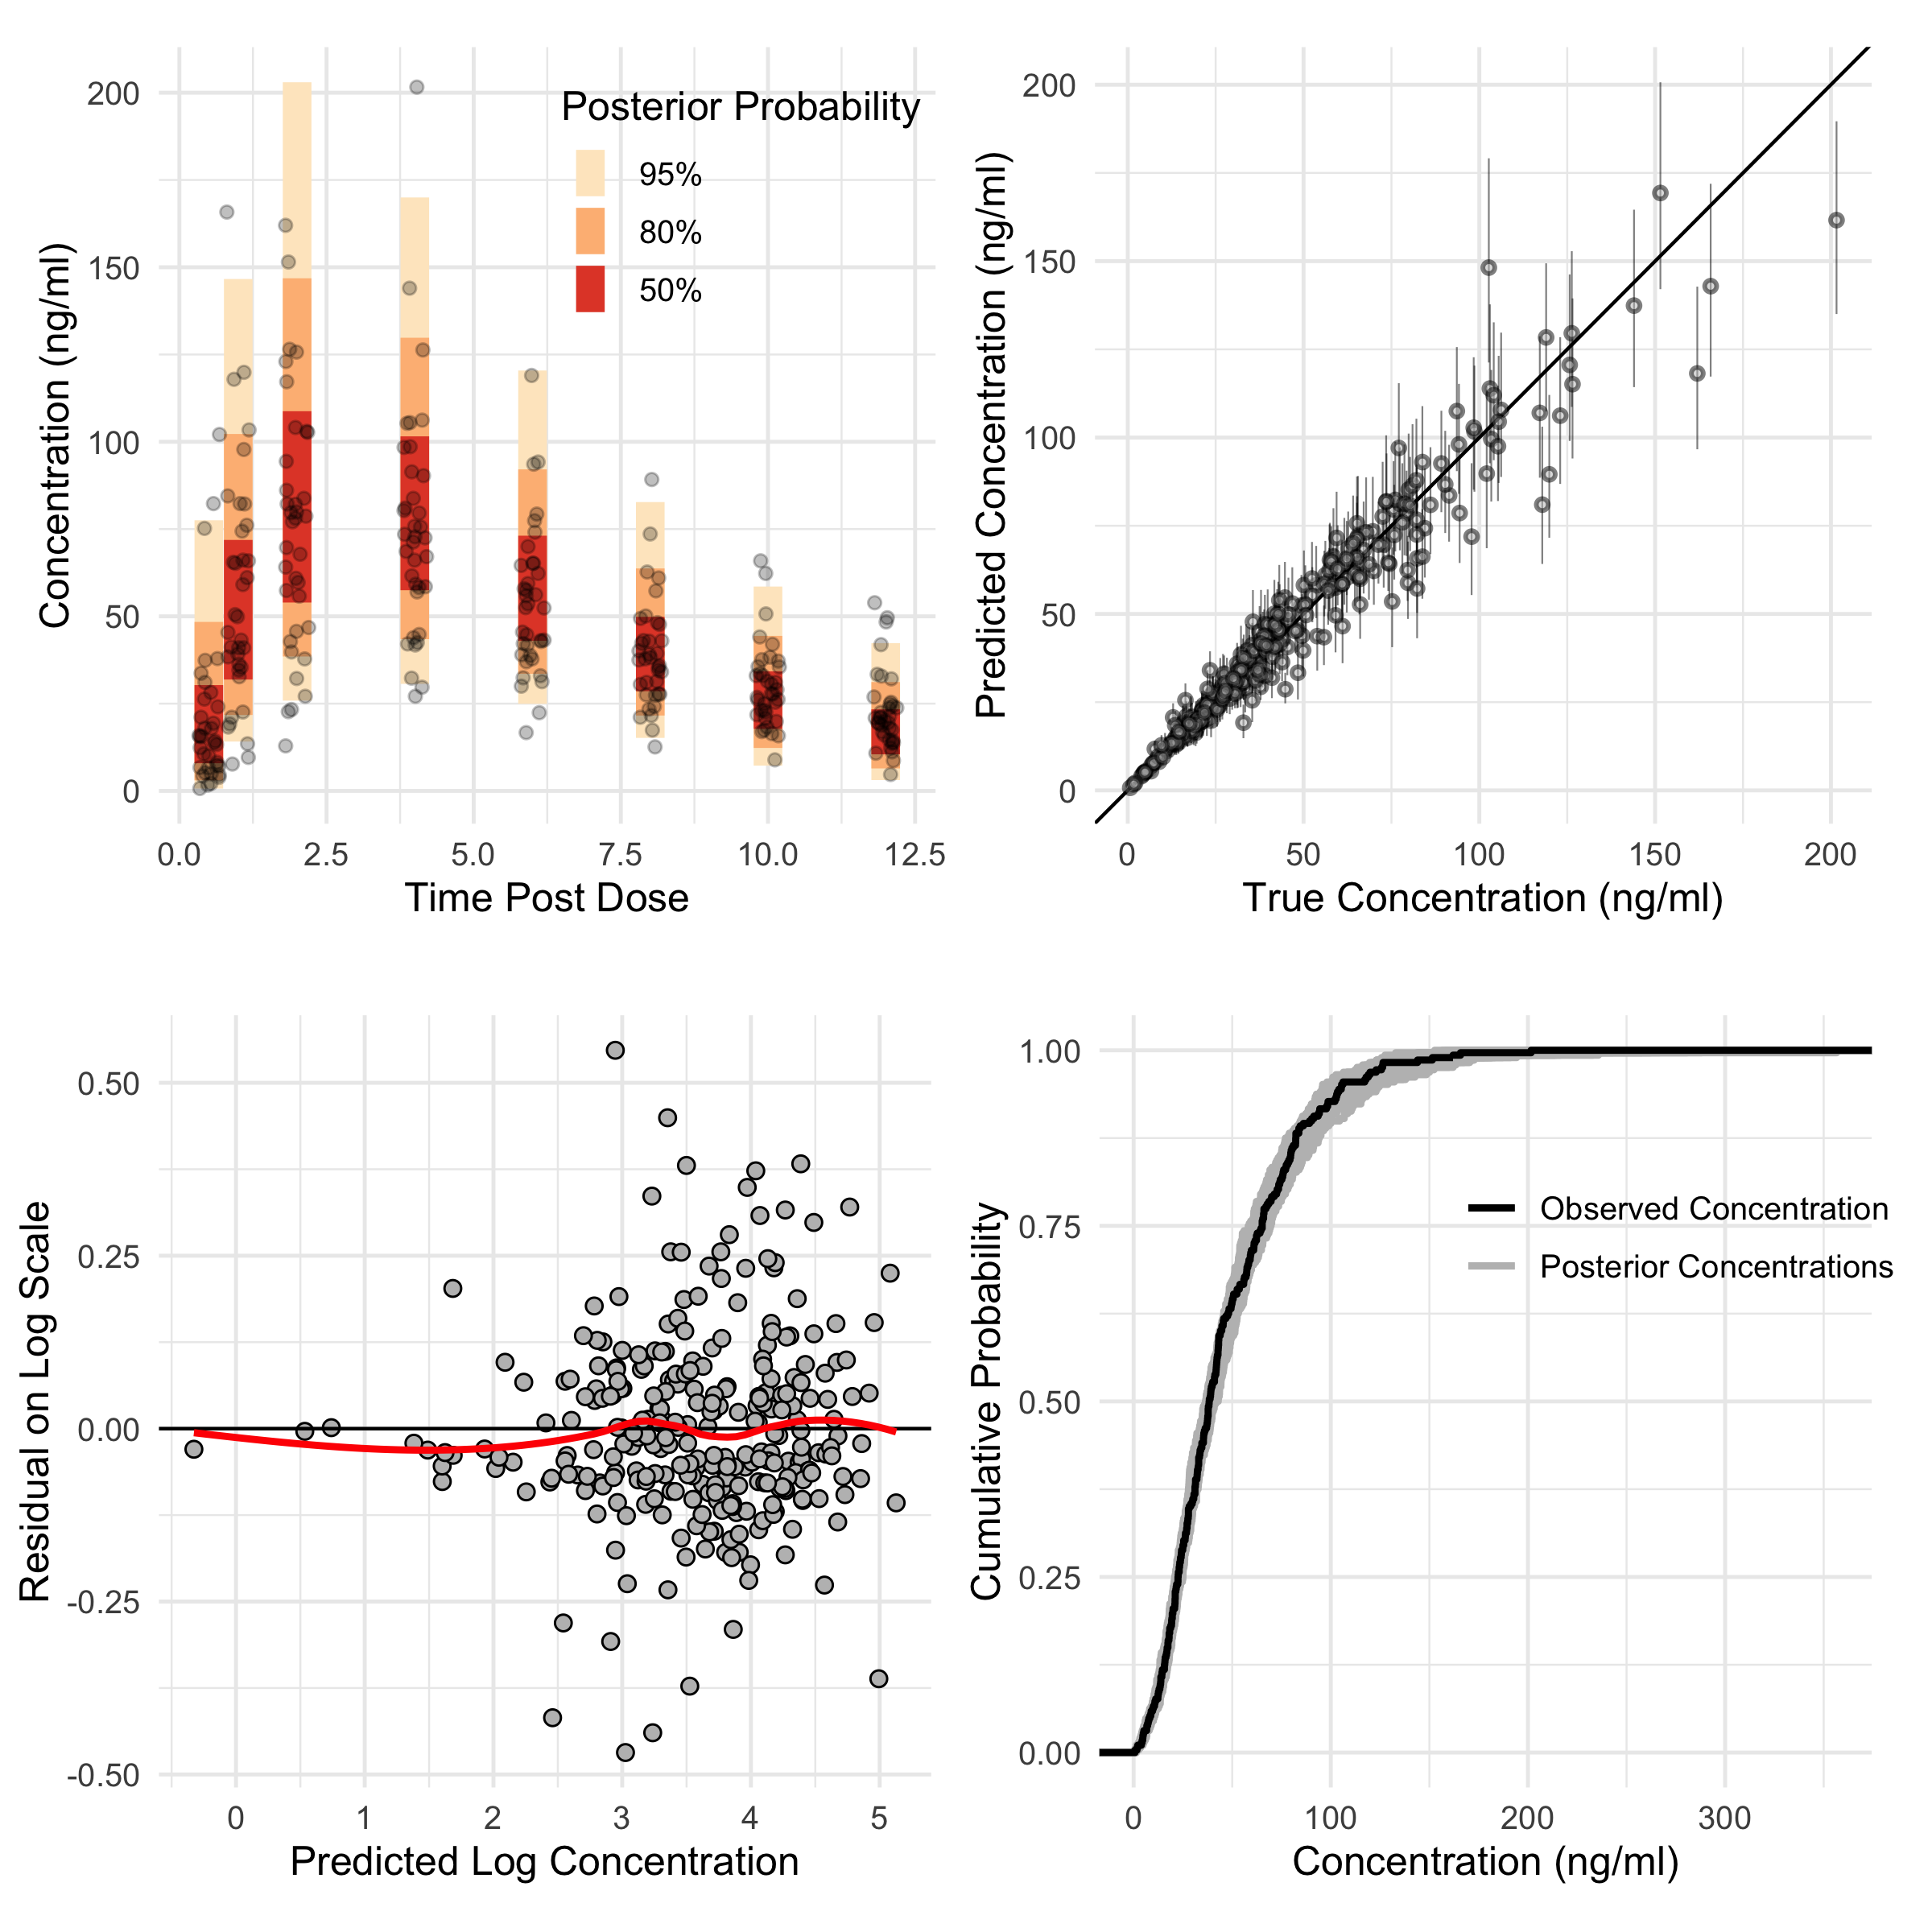
\includegraphics[width=0.9\linewidth]{figs/diagnostics}
	\caption{Diagnostic plots for our Bayesian model.  Top left shows the posterior predictive distribution plus observed data.  Data points gave been perturbed to prevent overlapping. Top right shows the predicted values along with accompanying 95\% equal-tailed posterior credible interval. Bottom left shows the residuals (on the log scale) between the observed concentrations and the posterior mean concentration, bottom right shows the cumulative density function for the observed data (black) as well as draws from the posterior predictive distribution (gray).}
	\label{fig:fig3}
\end{figure}


\begin{figure}
	\centering
	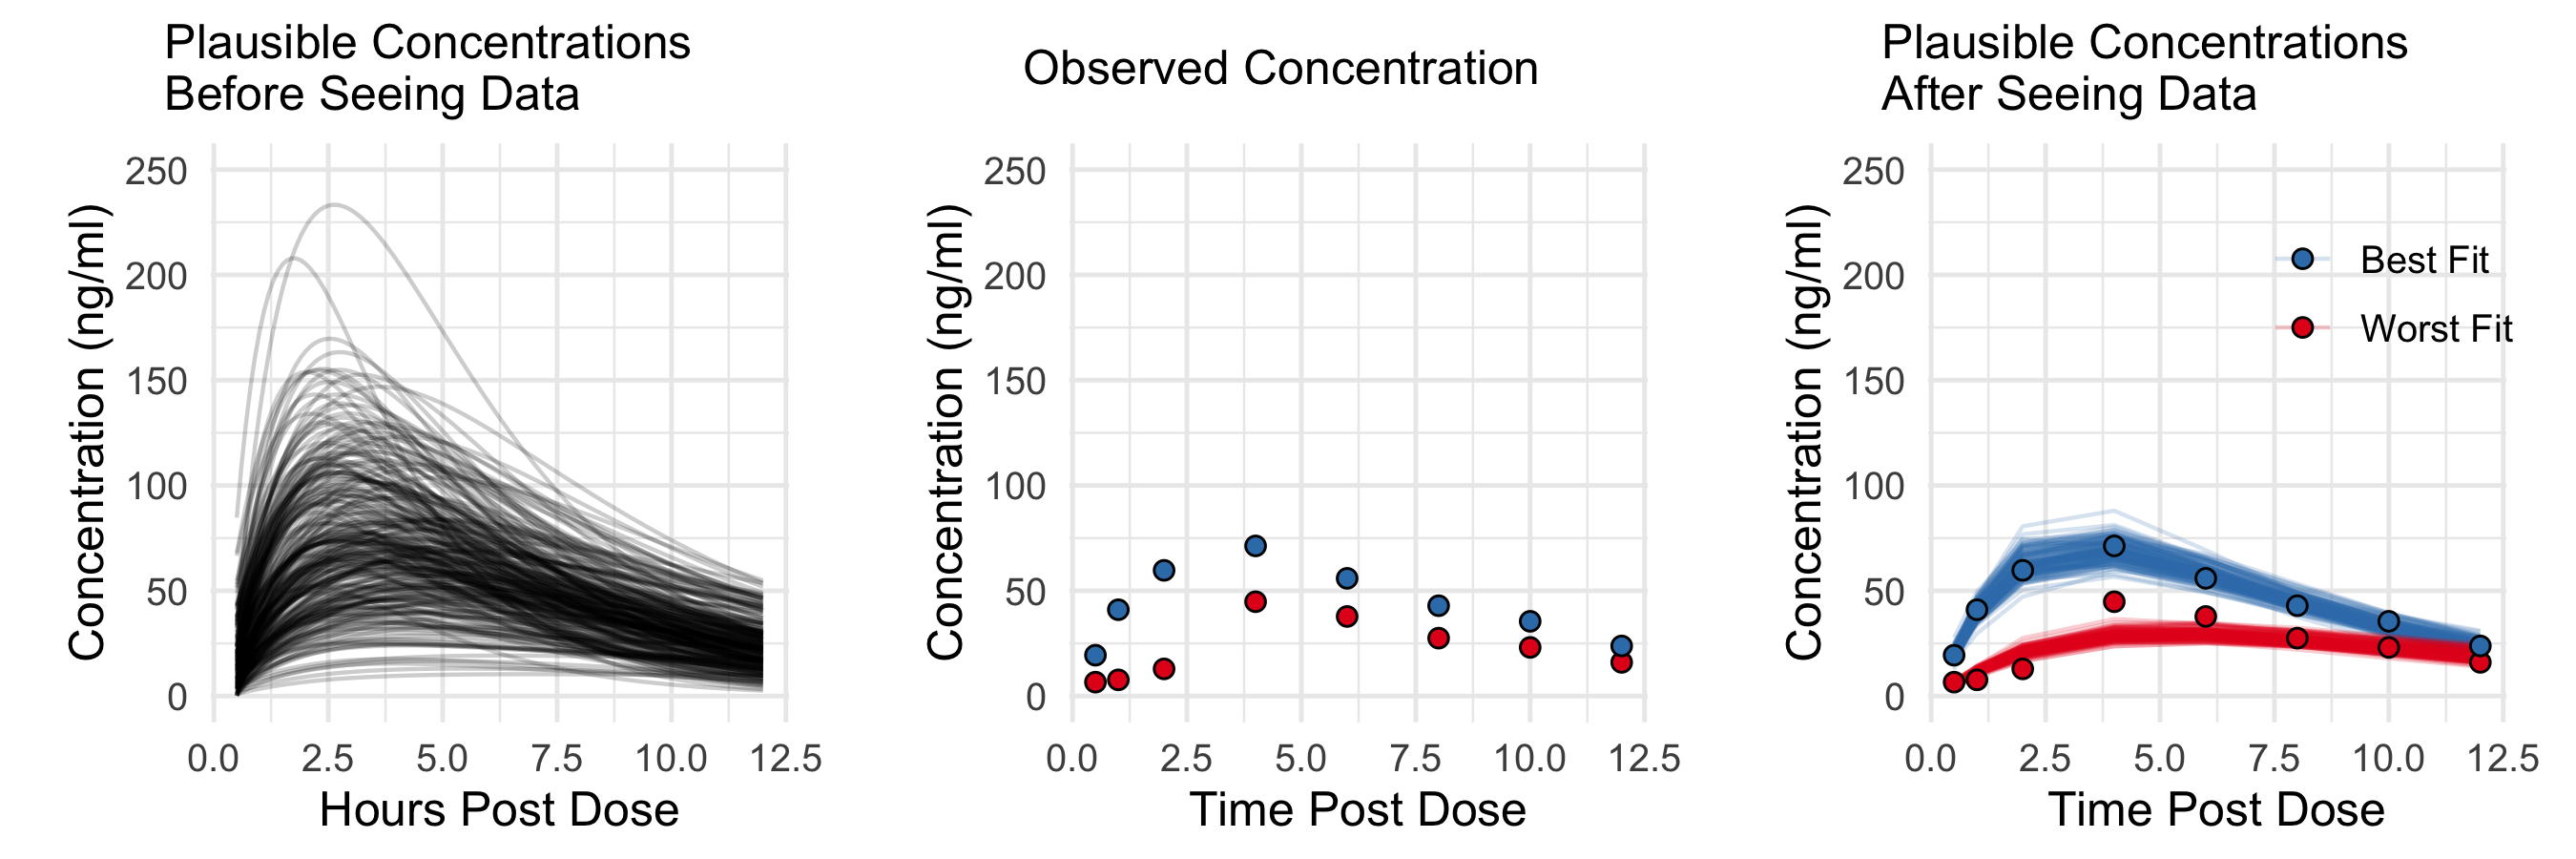
\includegraphics[width=\linewidth]{figs/fig3}
	\caption{The leftmost panel shows 250 draws from the prior defined in the previous section.  The center panel shows data from two patients who acieved the best (blue) and worst (red) model fit as measured through mean absolute percent error.  The rightmost panel shows 250 draws from the posterior for these patients.  Not shown here are the other 34 patients in our data, for which the model is also capable of performing predictions for. }
	\label{fig:fig4}
\end{figure}

\begin{figure}
	\centering
	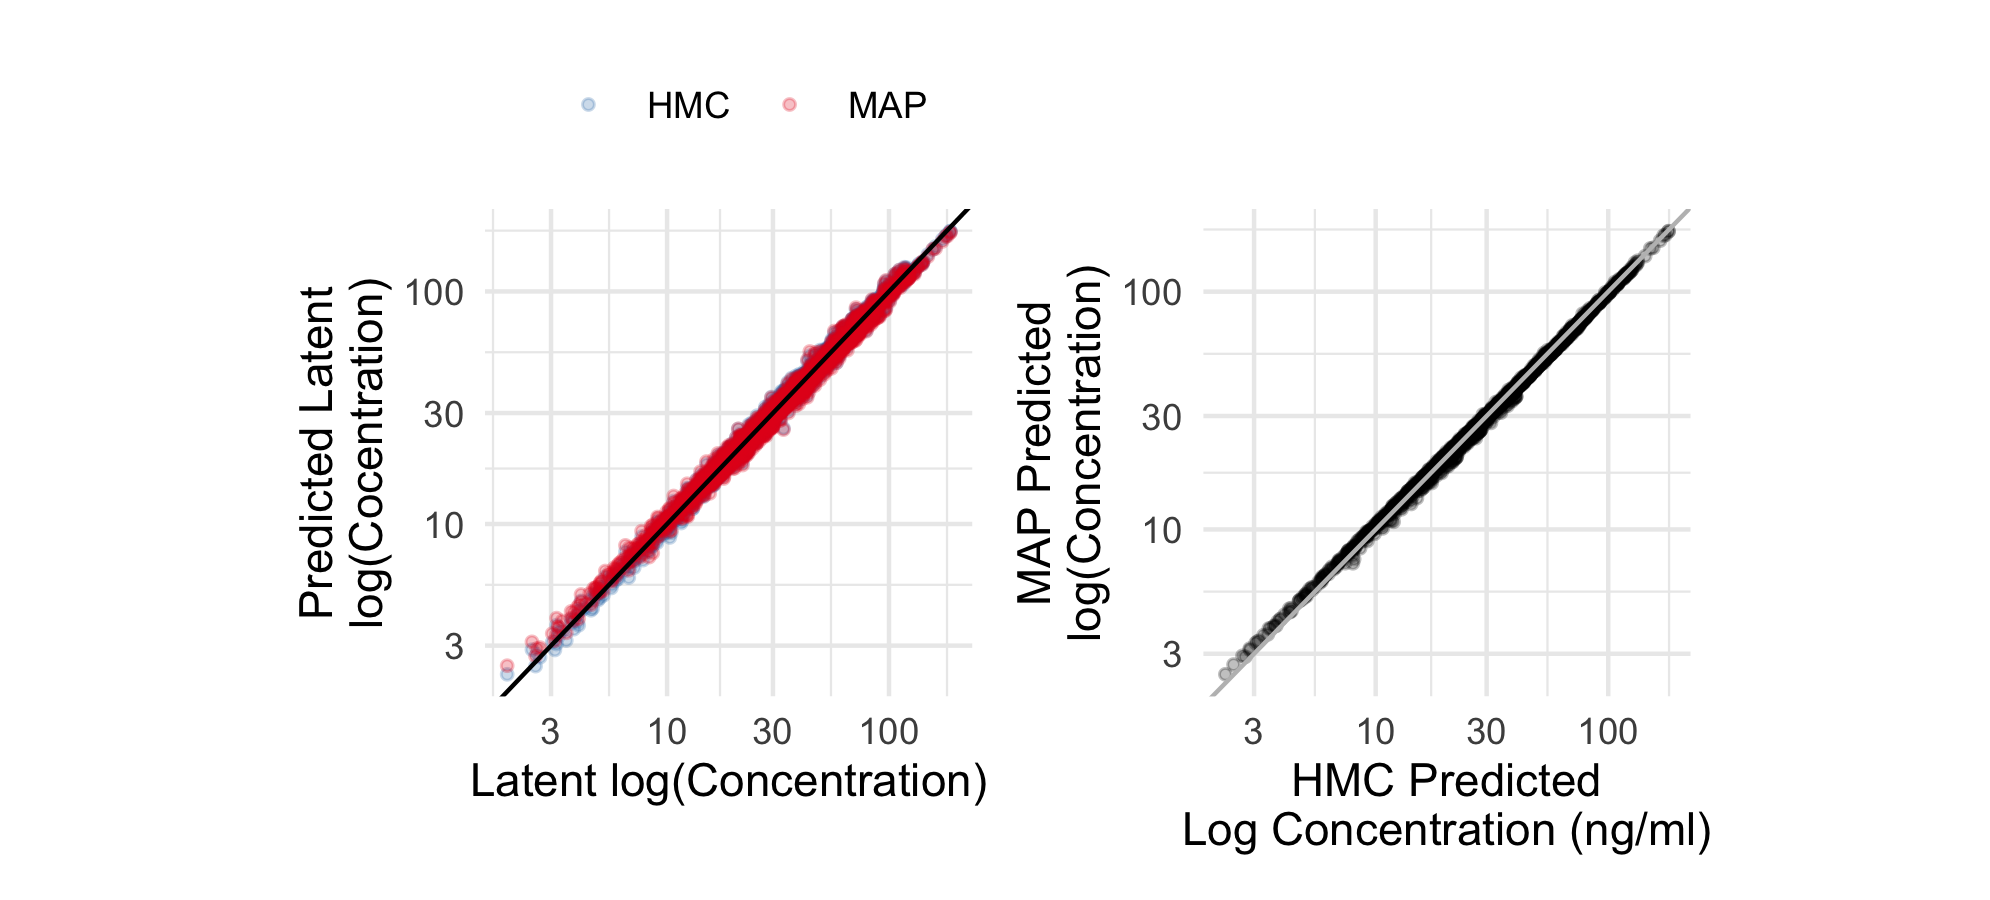
\includegraphics[width=1\linewidth]{figs/compare}
	\caption{Comparisons of fits obtained through HMC and MAP for simulated patients.  On the left, the two methods are compared to the true concentration values, and on the right the two methods are compared to one another.  The predictions are negligibly different to the eye and are also negligibly different as compared by Mean Squared Error (MSE), Mean Absolute Error (MAE), and Mean Absolute Percentage Error (MAPE).}
	\label{fig:fig5}
\end{figure}



\subsection*{Fit on Simulated Patients Using HMC and MAP}

Initial comparisons of predicted values indicate that both HMC and MAP yield similar predictions to one another, and similar predictions to actual values of unseen data (see \cref{fig:fig5}).  Examining predictions alone, it would seem that HMC and MAP are equivalent, or at the very least similar enough so as to not have strong preference for one over the other. When using posterior means, HMC results in lower prediction error on unseen data (see \cref{table2}) as measured with Mean Squared Error (MSE), Mean Absolute Error (MAE), and Mean Absolute Percentage Error (MAPE), but these are not stark differences. Estimates of posterior uncertainty between MAP and HMC can however vary a great deal. Shown in \cref{fig:fig6} are 19 of the 100 simulated patients which have a MAP equal tailed posterior interval at least 50\% larger as compared to their HMC equal tail posterior interval at the widest point. We note that while not shown explicitly, unobserved concentrations lie entirely within the HMC and MAP posterior intervals.



\begin{table}
	\centering
\begin{tabular}{|c|c|c|}
	\hline 
	& HMC & MAP \\ 
	\hline 
	MSE (SD) & 6.67 (15.93) & 8.57 (19.93) \\ 
	\hline 
	MAE (SD) & 1.71 (1.94) & 1.97 (2.17) \\ 
	\hline 
	MAPE (SD) & 0.04 (0.03) & 0.05 (0.03)\\ 
	\hline 
\end{tabular} 
\caption{Comparison of HMC and MAP on three loss functions common in pharmacokinetics:  Mean Squared Error (MSE), Mean Absolute Error (MAE), and Mean Absolute Percentage Error (MAPE).  The loss was computed on samples not seen by our model.  Included in parentheses are the standard deviations of the loss values.}
\label{table2}
\end{table}

%\begin{figure}
%	\centering
%	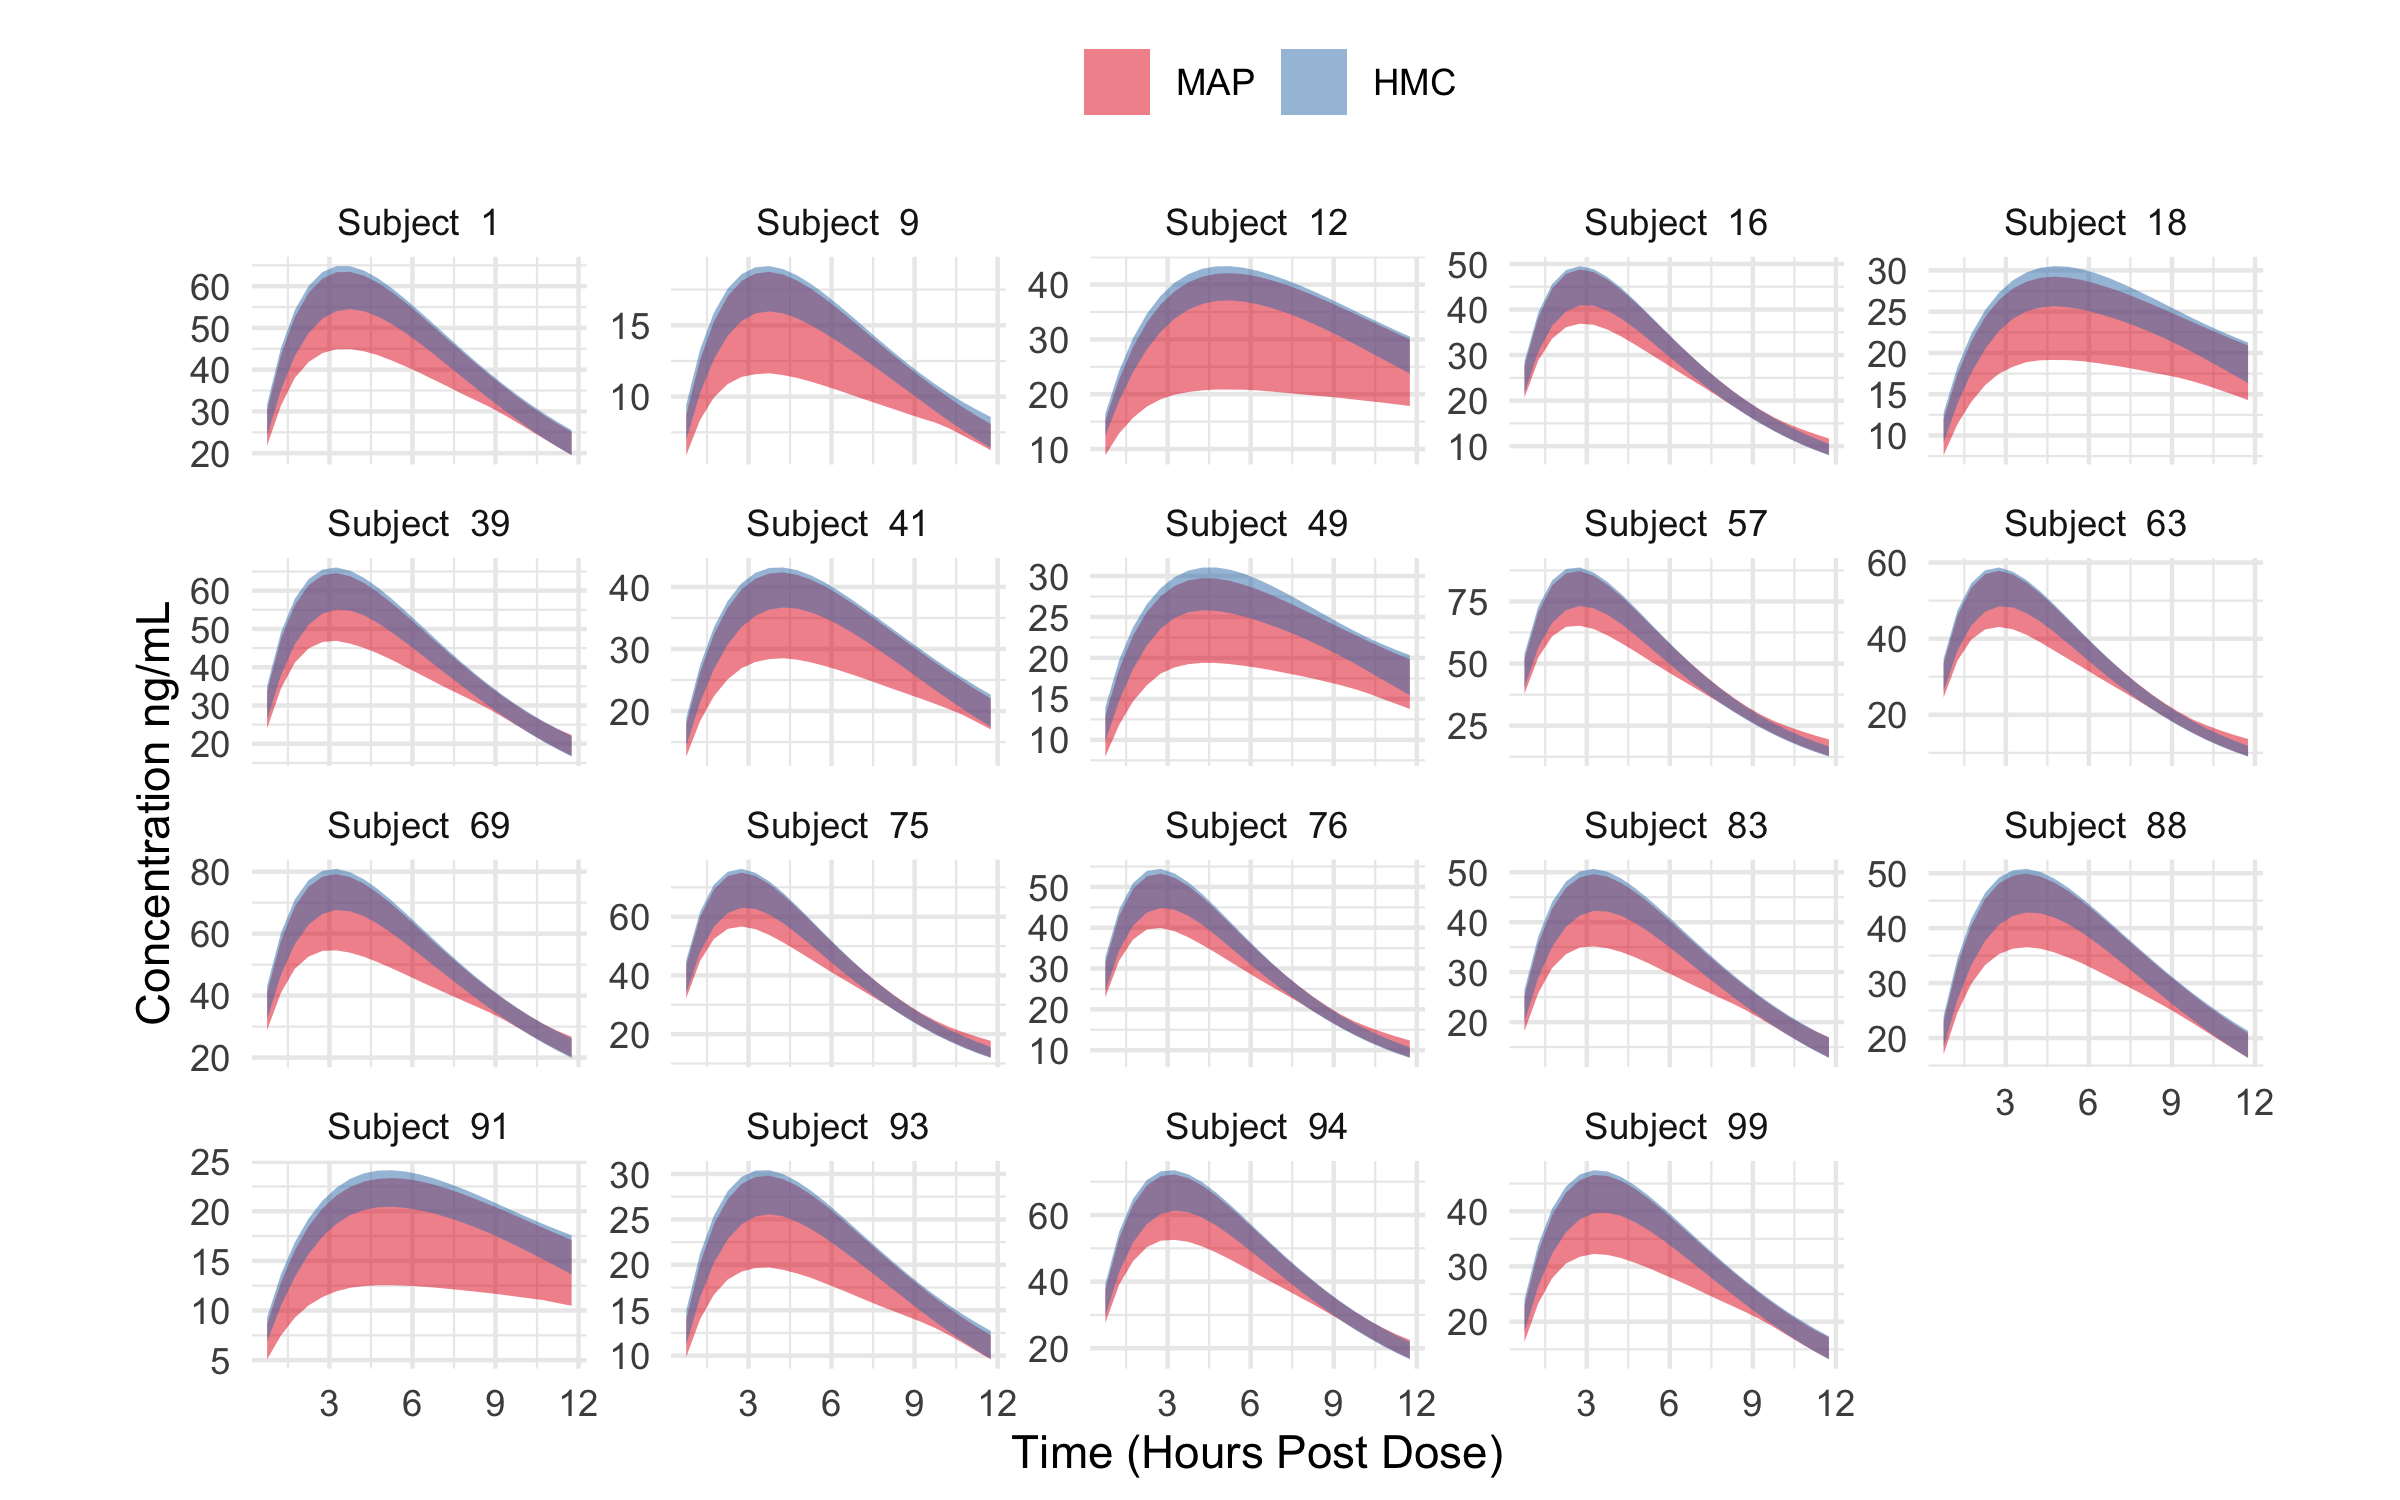
\includegraphics[width=1\linewidth]{figs/intervals}
%	\caption{Comparisons of equal tail posterior intervals from MAP and HMC. Note that the concentration scales differ from subplot to subplot.  Selected patients are those which have a MAP posterior interval at least 50\% as wide or wider than their HMC interval.  In many simulated subjects.}
%	\label{fig:fig6}
%\end{figure}
\clearpage
\begin{sidewaysfigure}[h!]
\centering
	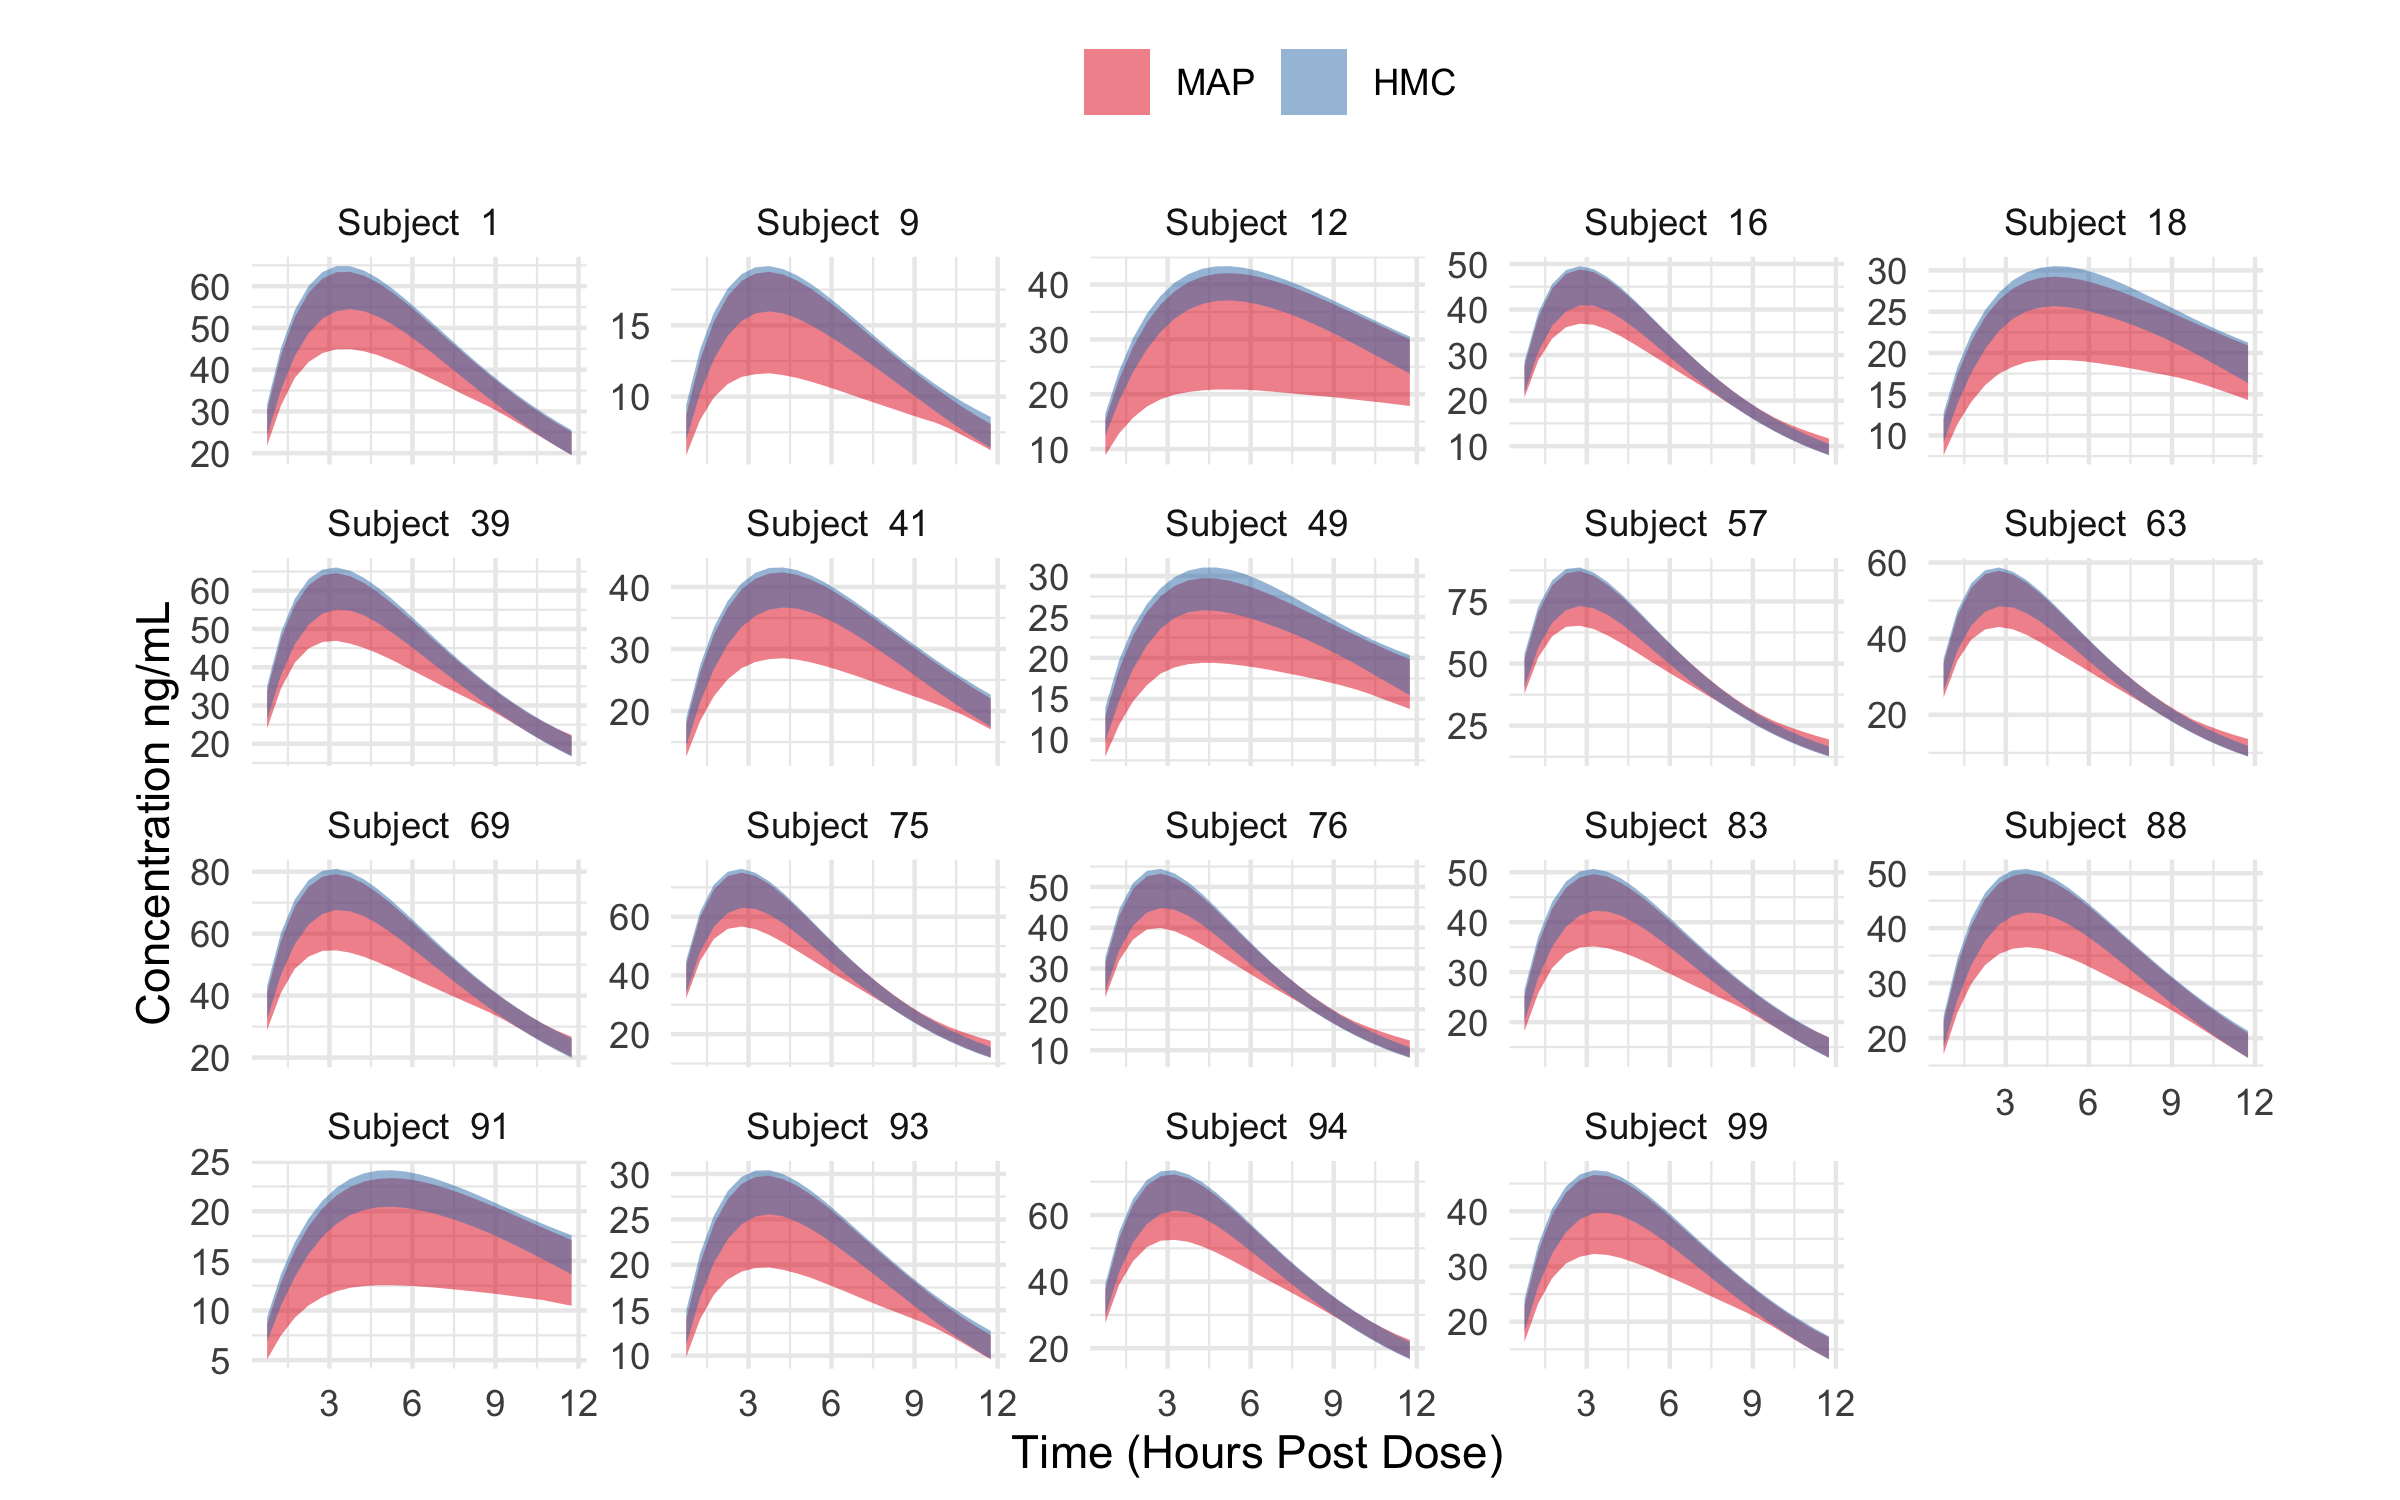
\includegraphics[width=1\linewidth]{figs/intervals}
	\caption{Comparisons of equal tail posterior intervals from MAP and HMC. Note that the concentration scales differ from subplot to subplot.  Selected patients are those which have a MAP posterior interval at least 50\% as wide or wider than their HMC interval.}
	\label{fig:fig6}
\end{sidewaysfigure}
\clearpage

\subsection*{Difference in Estimated Dose To Achieve Target Risk}


By inverting the risk curve, we can obtain dose size as a function of risk.  Shown in \cref{fig:fig7} are the differences between doses computed from HMC and MAP posteriors to achieve the indicated level of risk.  The left panel shows the difference in doses in order to achieve a concentration of at least 20 ng/ml 12 hours post dose. For a majority of patients, MAP and HMC agree to within 1 mg though some pseudopatients see a much larger dose recommendation by HMC than by MAP.  The right panel shows the difference in doses in order to achieve a max concentration of 80 ng/ml.  MAP tends to always recommend larger doses than HMC for this scenario, with the difference between recommended doses becoming larger as the desired risk becomes smaller.

\begin{figure}[h!]
	\centering
	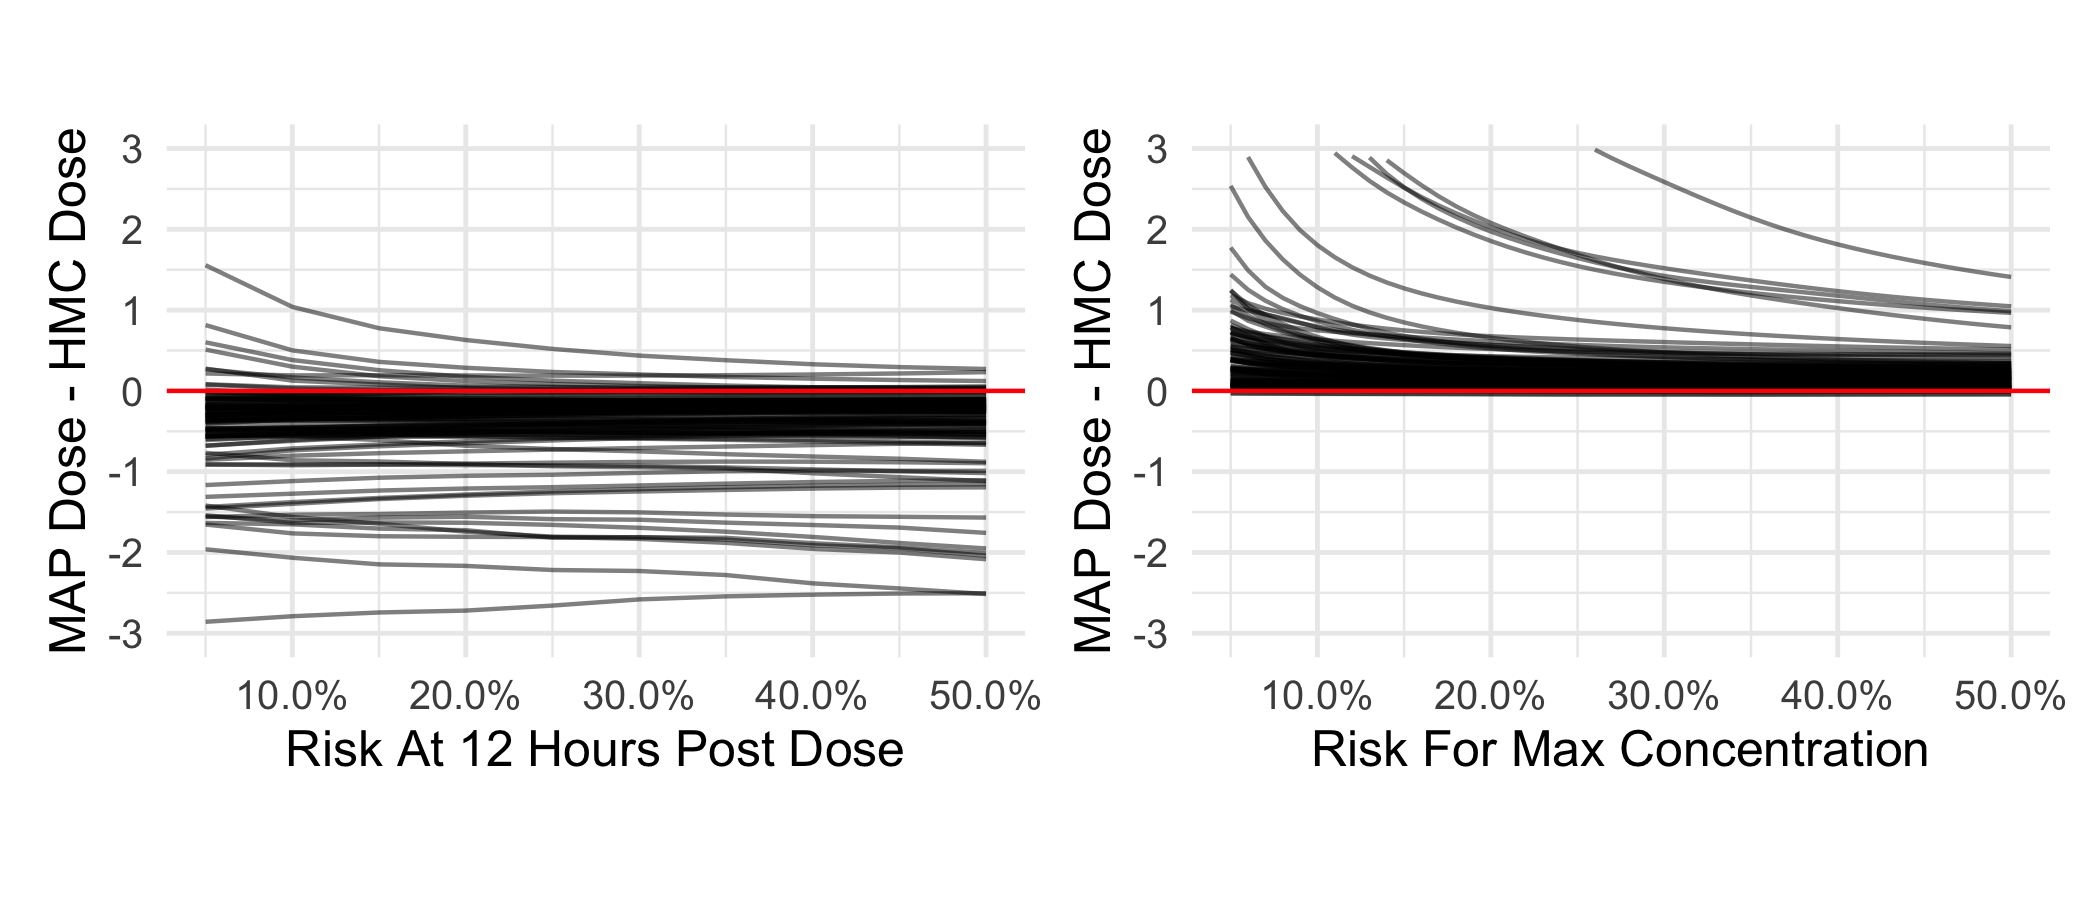
\includegraphics[width=\linewidth]{figs/experiments}
	\caption{Left: Differences between the estimated doses from MAP and HMC to achieve the indicated risk of having a concentration of apixiban smaller than 20 ng/ml at 12 hours post dose. Each line corresponds to one of the 100 pseudopatients. HMC tends to recommend larger doses than MAP to achieve a desired risk of having the patient's concentration at 12 hours post dose be below 20 ng/ml. This tendency to recommend larger doses is consistent across desired risk levels.  Right: Differences between estimated doses from MAP and HMC to achieve the indicated risk of having a max concentration smaller than 80 ng/ml.  Some pseudopatients see dose recommendation differences as large as 10 mg and are thus cut off by the y axis limits. Red lines indicate where the two methods would perfectly agree.}
	\label{fig:fig7}
\end{figure}


\subsection*{Calibration for Dosing Decisions}

Since all pseudopatients were simulated, the true concentration function as a function of the dose size (\cref{eq:eq_1}) was known.  To further compare HMC and MAP for decision making, we took estimated dose size to achieve a desired risk and computed what the concentration curve under the recommended dose size.  We could then compute the number of pseudopatients which actually exceeded the threshold, thus allowing us to examine the calibration of HMC and MAP.  The calibration curves for HMC and MAP for both experiments are shown in \cref{fig:fig8}.

In the first experiment (left of \cref{fig:fig8}), HMC is better calibrated than MAP.  This means that when a dose is selected, in order to a achieve a risk of being below 20 ng/ml at 12 hours post dose of $r$, approximately $r \times 100$ pseudopatients have a true concentration function which is smaller than 20 ng/ml at 12 hours post dose. In contrast, MAP is poorly calibrated, and sees more pseudopatients failing to exceed the 20 ng/ml threshold than was desired.  Calibration in our second experiment again shows than HMC is better calibrated than MAP, but calibration seems to become worse as the desired risk becomes larger.  When we use dose sizes recommended by MAP to achieve a 50\% probability of exceeding the 80 ng/ml threshold, only 26\% of pseudopatients actually have a max concentration which exceeds the threshold.


\begin{figure}[h!]
	\centering
	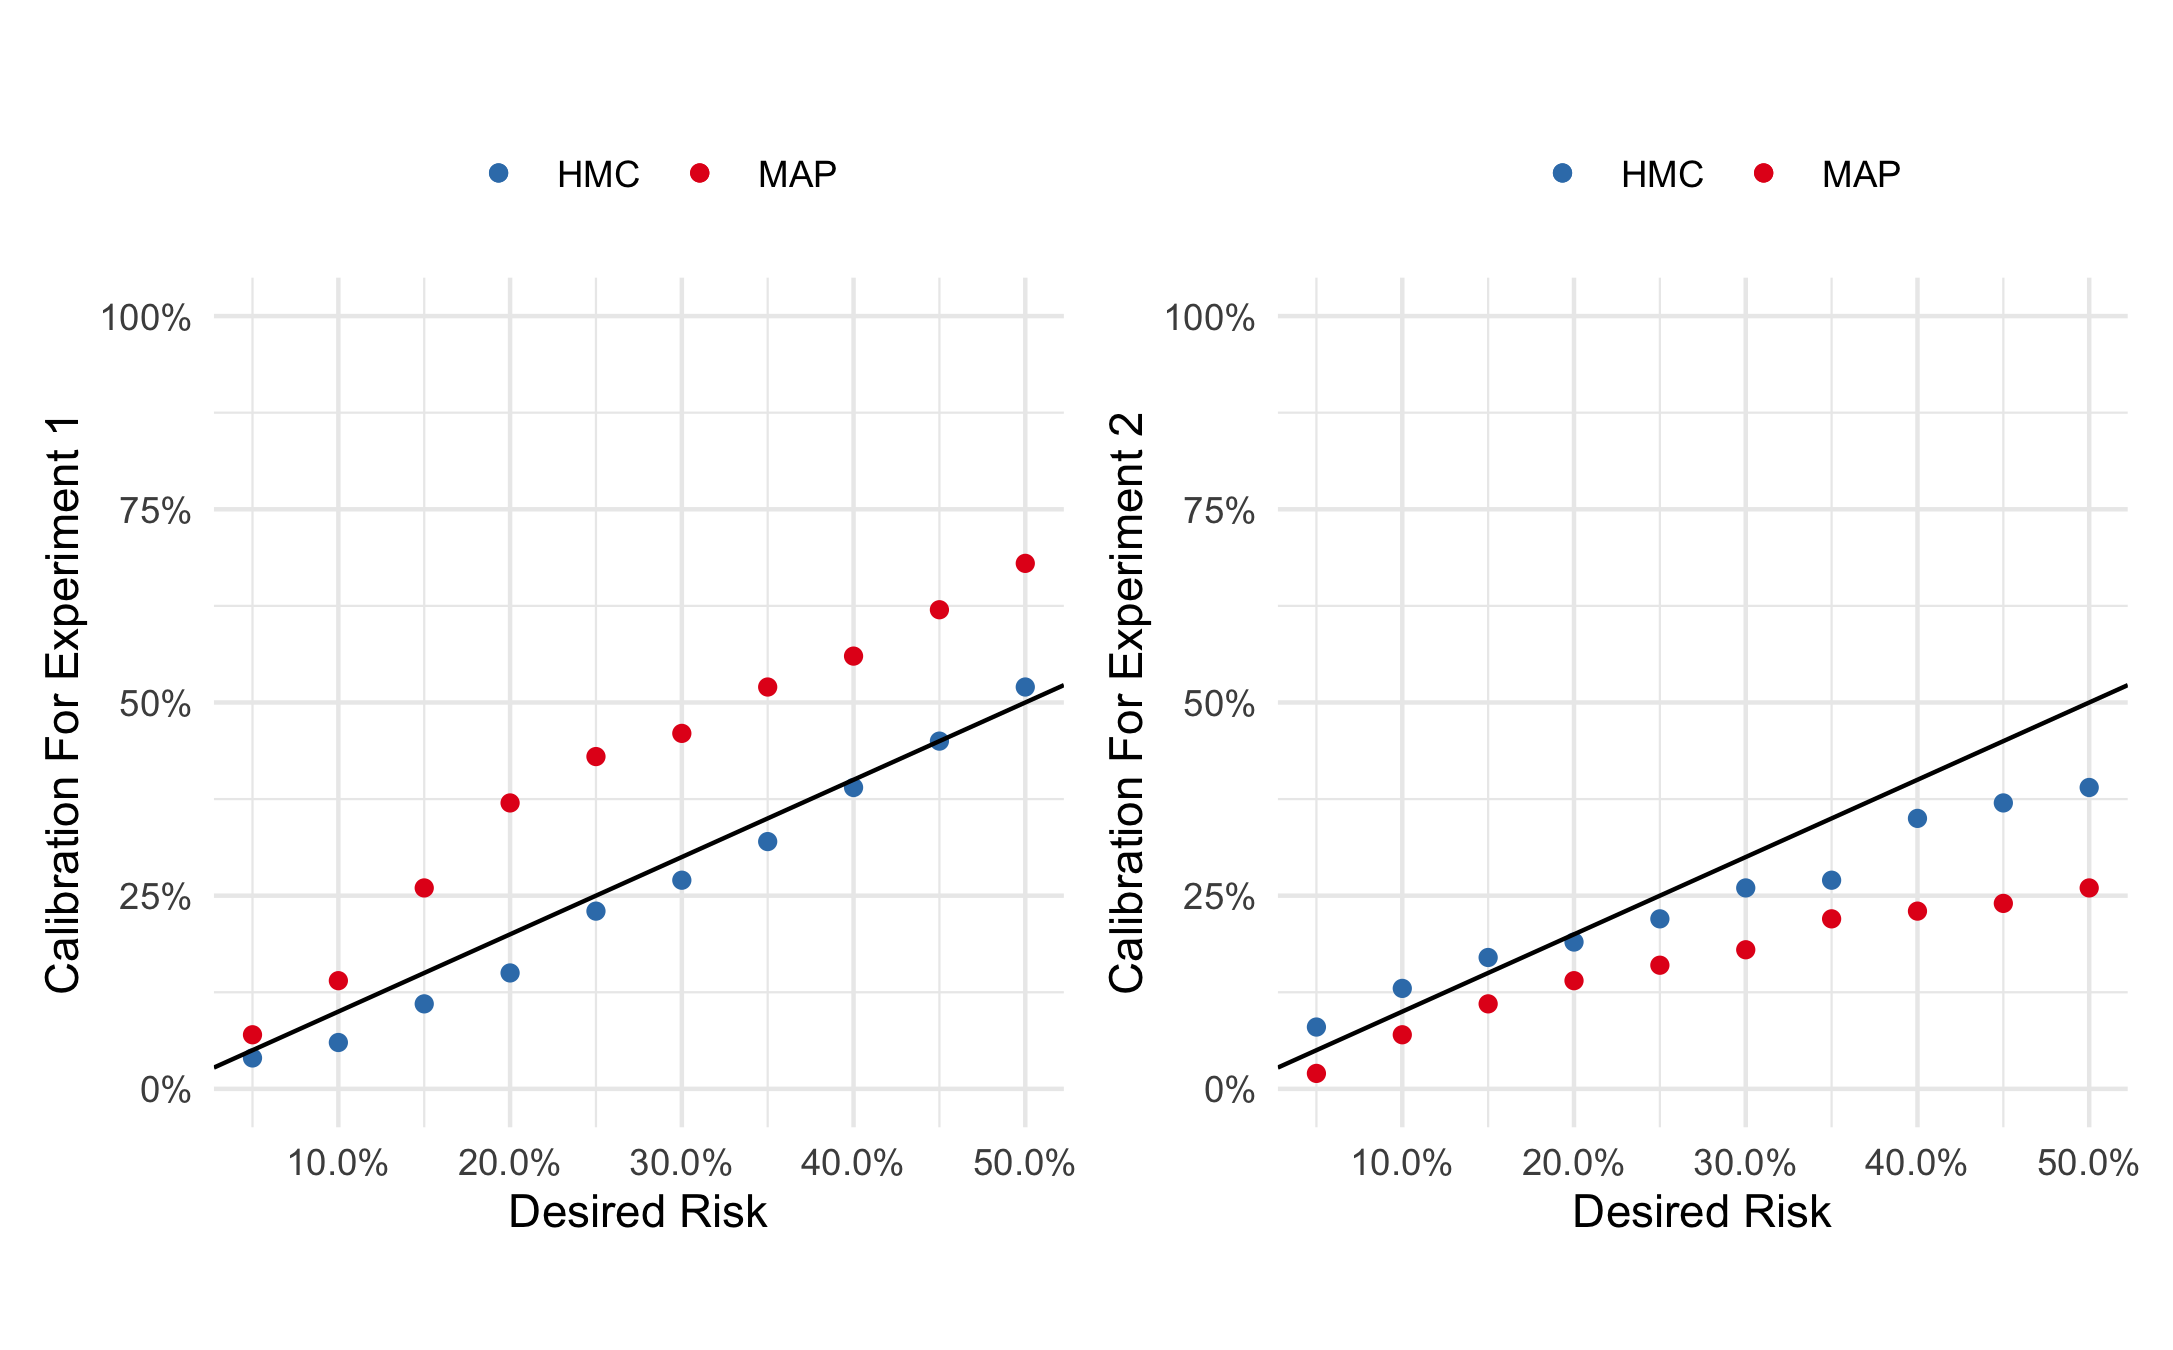
\includegraphics[width=\linewidth]{figs/fig8.png}
	\caption{Left: Calibration curves for assessing risk of being below 20 ng/ml.  Each dot represents the proportion of the 100 pseudopatients which fail to exceed the 20 ng/ml threshold.  When doses are chosen from samples obtained via HMC, then probabilities are well calibrated. When doses are chosen from samples obtained via MAP, more pseudopatients fail to exceed the threshold than were specified.  Right: Calibration curves for assessing risk of the max concentration being below 80 ng/ml. HMC appears to be better calibrated than MAP, though the calibration could stand to improve.}
	\label{fig:fig8}
\end{figure}




\section{Discussion}

While prediction errors of the point estimates produced by MAP and HMC are very similar as measured by 3 losses common to pharmacokinetic research, they each produce very different estimates of uncertainty.  Such estimates are necessary for decision making under uncertainty, where an expected loss is computed over a posterior distribution.  In this study, for a given dose, MAP assigns a significant amount of probability mass to concentrations which are far lower than the concentrations considered plausible by HMC.  The extent to which this discrepancy would change decisions depends on the loss function, but we see substantial differences in our two example experiments for personalized dosing.  The difference in uncertainty between MAP and HMC results in small disagreement for dose size for the majority of patients, but very large disagreement for a sizable minority of about 20\%. The observed difference in uncertainty for the concentration function between MAP and HMC are likely due to discrepancies in uncertainty over the individual PK parameters: Each of the 19 pseudopatients in \cref{fig:fig6} see MAP and HMC disagree strongly on posterior uncertainty for the parameters $k_a$ and $k_a$.  MAP lends credence to higher values of $k_a$ and lower values of $k_e$ as compared to HMC. The differences in uncertainty in these parameters is likely the cause of the observed difference in uncertainty in concentration levels. This translates into much wider equal-tailed posterior intervals for concentration using MAP, with 19 out of 100 patients having an MAP equal tailed posterior credible interval at least 50\% as wide or wider at their widest point than their HMC equal tailed posterior interval. For each of these 19 patients, MAP appears to have a lower interval estimate far below that of HMC, making it appear as if lower predicted concentrations are probable. This in can make a given proposed dose appear risky in terms of allowing concentration to fall too low; which in turn leads to an increase in recommended dose when the model is asked for a dose that bounds this risk.

While the posterior distribution for this model is too complex to be analyzed analytically, there are good theoretical reasons to prefer HMC over MAP when analysts seek the posterior expectation of some function of parameters. These reasons are nicely summarized by \cite{Betancourt2017-ak}, but can be distilled into the fact that expectations are computed over volumes, and in high dimensional space there exists more volume away from the mode than in a neighbourhood around it. Because the volume near the mode is so small, these regions of parameter space contribute negligibly to expectations.  Instead, regions of parameter space where the product of probability density and volume is large should contribute more to expectations, and this is where our chosen method should be focussing its computational power.  Hamiltonian Monte Carlo does exactly this.

Neither HMC nor MAP provide perfect representations of the posterior, and discrepancies between the two methods are expected. However, the degree of discrepancy observed in this study and its impact on dosing decisions reveals that these techniques are not interchangeable. On reason for the observed difference might be an insufficient number of observations.  However, with 24 equally-spaced observations per each of the 100 simulated patients, this simulation study represents an extremely optimistic (and likely unrealistic) best case scenario. Even specialized studies of pharmacokinetics would collect fewer samples from fewer patients, and even less data collection is practical in clinical practice. Hence, even if MAP and HMC were to converge to each other with enough data, this amount of data is not available in practice. Another possible reason could be the chosen priors and/or the likelihood, but the model used was identical for both inference methods and had strong priors informed by existing pharmacokinetic data.  We note also that although our models did not account for patient covariates, a secondary analysis was performed in which patient level pharmaokinetic parameters were regressed onto patient covariates.  In this analysis, we observed the same disagreement in model uncertainty as shown in \cref{fig:fig6}.

%By performing the summarization of the posterior using the same data, generated from a model fit on real pharmacokinetic observations, and using strong and informative priors, we strongly believe that this observed difference is due to the differences between methods. However, that is not to say that this is the case across all models and prior configurations.  The prior we propose is purposefully uninformative about the ratio of the elimination and absorption rate constants, so as to investigate a likely scenario in which prior information is available for some but not all of the model parameters.  Were this prior to be strongly informed, we highly suspect that the observed differences between HMC and MAP would attenuate.  This raises important questions about model specification and the degree to which practitioners can afford to be uncertain about model parameters.

\section{Conclusion}
We have presented a new Bayesian model for apixaban pharmacokinetics and an induction dosing model for apixaban based on desired trough concentration level after a first dose. We have also presented a simulation study demonstrating that inferences made via MAP and HMC lead to very different dosing strategies; from this simulation study, we derive some general conclusions and guidelines for Bayesian PK modelling as applied to personalized medicine.

Bayesian modelling using informative priors provides a practical approach for developing personalized dosing strategies when data are limited. However, the evaluation of Bayesian models, particularly with informative priors, typically focuses on the model itself - are the priors plausible? Do posterior predictive checks look appropriate? In this work, we have demonstrated that the inference technique can have an impact on decision making that is as important as model fidelity, even when the impact on point prediction quality is minimal. Specifically, we have shown that MAP-based inference, which is very commonly used in pharmacokinetics, can lead to very different personalized dosing decisions than HMC-based inference, even in a well-validated model.

Studies using MAP for Bayesian inference in pharmacokinetic models have been published as recently as 2020.  The speed and similarity to maximum likelihood makes MAP an attractive and familiar approach as compared to HMC, which can take several minutes to return samples and can use quite complex mechanisms to draw from the posterior. The aforementioned studies have largely focused on point predictions of latent concentrations where, as we have shown, MAP and HMC yield similar results. However, when uncertainty information is used for decision-making, MAP and HMC can lead to very different outcomes.

We recommend that if practitioners do use MAP, that they also compare model results with HMC.  Libraries exist to perform HMC in a variety of languages including R, python, and Julia, making HMC widely accessible.  Use of these libraries has the added benefit of making analysis more transparent and reproducible for the community at large.


\bibliography{references}



\end{document}
